\label{chpt:introduction} % for referencing this chapter elsewhere, use \ref{chpt:label}
\lhead{\emph{Background, context, and motivation}} % This is for the header on each page - perhaps a shortened title

Cataclysmic Variable (CV) systems consist of a white dwarf primary, and a lower mass red dwarf secondary star. The two are in extremely close proximity, such that the outer layers of the secondary are gradually accreted onto the white dwarf; this mass transfer process affects the evolution of both stars, in particular the donor, and is the main driving mechanism for the evolution of the system as a whole.
The mass transfer also gives rise to two more observable features of a CV: an accretion disc around the white dwarf, and a shock-heated bright spot region where accreted donor material impacts the outer rim of the disc \citep{warner1995,hellier2001}. Figure~\ref{fig:introduction:CV schematic} shows a schematic of this structure.
\begin{figure}
    \centering
    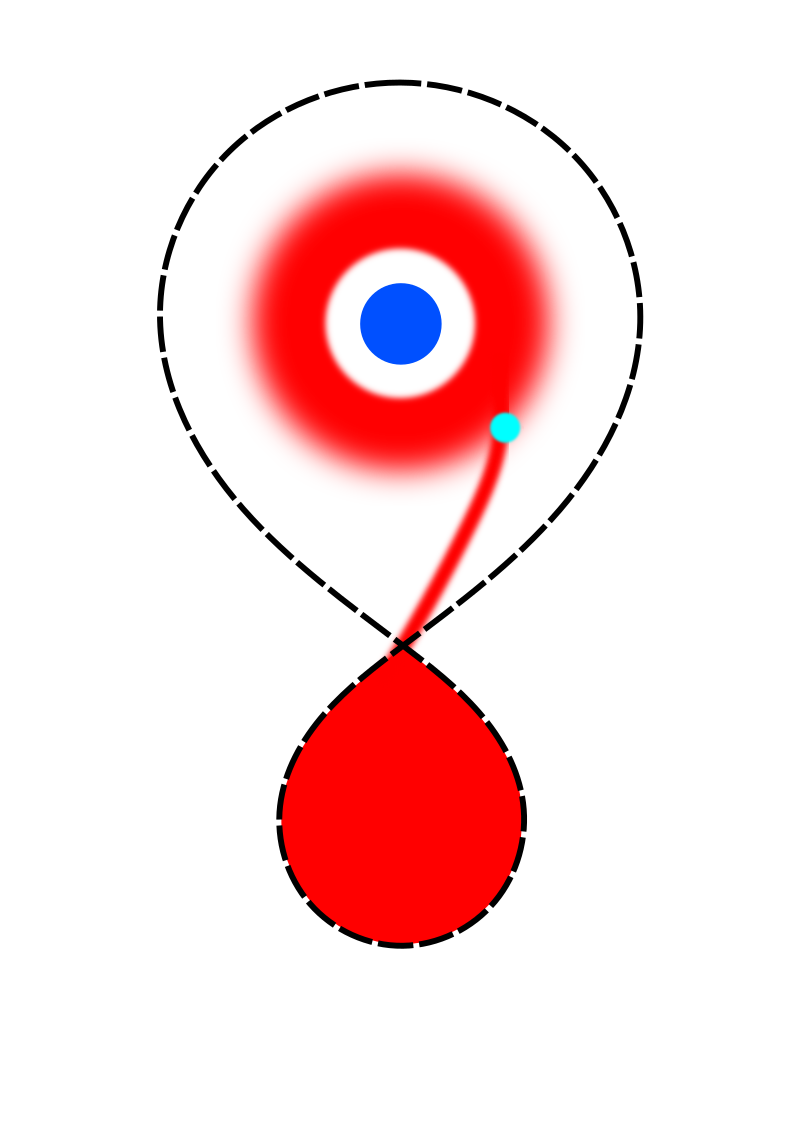
\includegraphics[width=0.6\textwidth]{figures/introduction/CV_schematic.png}
    \caption{A schematic of the structure of a CV, not to scale. The {\bf black dashed line} outlines each Roche lobe. The {\bf dark blue circle} is the white dwarf and is surrounded by its accretion disc. The {\bf lower red teardrop} is the secondary star, and is connected to the donor via the mass stream. The {\bf light blue spot} where the mass stream meets the disc is the bright spot impact region.}
    \label{fig:introduction:CV schematic}
\end{figure}

Systems actively undergoing mass transfer are important to our understanding of stellar evolution. A diversity of stars will experience a mass transfer phase, and losing mass strongly influences a stars' evolutionary path and must be accounted for (e.g. \citealt{renzini1981, smith2014} for single stars, or \citealt{hurley2002} for binaries). Of such systems, CVs in particular are interesting as modelling their eclipse lightcurves can yield precise, independant measures of both stars' mass and radius \citep{wood1986,Littlefair2008,Savoury2011}. Further, since the donor stars' evolution is dominated by its mass loss, CVs provide a window into binary evolution \citep{knigge2006}.
The mass loss itself is driven by poorly-understood mechanisms, classically attributed to stellar magnetism and gravitational waves, that can also be probed using CV observation and modelling.

Since CVs are binary stars, in the case of eclipsing systems it is possible to make direct observations of orbital separations, stellar masses, and radii. This lends some powerful diagnostics, in addition to parameters accessible with more general techniques such as spectroscopic analysis.
The ability to thoroughly characterise CVs makes them an excellent test-bed for binary modelling, and the complex processes that contribute to their evolution.
Unfortunately, whilst reasonably accurate semi-empirical modelling of most of the CV evolutionary track and population distribution have been now possible for more than a decade (e.g. \citealt{knigge11,Paxton_2015}), the field has yet to produce physically motivated theoretical models capable of accurately reproducing either the CV population distribution or complete evolutionary track, indicating some shortfalls in our understanding \citep{schreiber2015,Schreiber2016}.
Of most significance to this work is the problem of missing Angular Momentum Loss (AML), where CVs with low mass donor stars appear to be losing angular momentum much faster than our models predict \citep{Schreiber2016}. This first chapter will summarise the current understanding of CV formation and evolution, and will focus on the issues with CV evolutionary models.


\section{Roche geometry}
\label{sect:introduction:Roche geometry}

Before discussing the formation, structure, and evolution of CVs, it is first critical to understand Roche lobes.
In a two-body orbital system, the Roche potential of a point is an effective potential in the non-inertial, co-rotating frame of reference. It is given by the sum of the gravitational potential energies due to the two masses, and the potential energy arising from centrifugal force. This can be described mathematically for each position vector:
\begin{equation}
    {\bf \phi} = -\frac{G M_1}{|{\bf r - r}_1|} - \frac{G M_2}{|{\bf r - r}_2|} - \frac{1}{2}({\bf \Omega} \times {\bf r})^2
\end{equation}
Where $\phi$ is the Roche potential, G is the gravitational constant, $\bf r$ is the position vector being considered relative to the centre of mass, and $\bf \Omega$ is the angular momentum vector of the binary. $M_{1,2}$ and ${\bf r}_{1,2}$ are the masses and position vectors of the two orbiting bodies. measured from the centre of mass. Figure~\ref{fig:roche} shows this graphically.
\begin{figure}
    \centering
    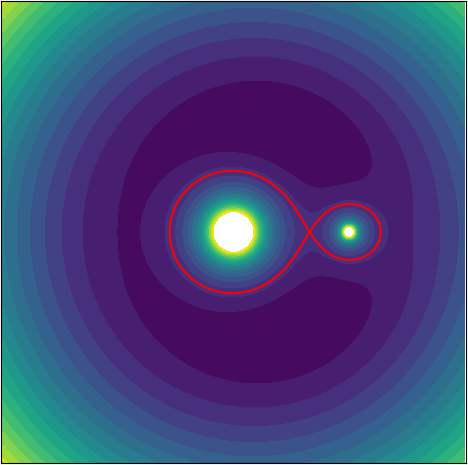
\includegraphics[width=.6\columnwidth]{figures/introduction/roche.png}
    \caption{Showing the Roche potential in the neighbourhood of the binary system, with the more massive primary star on the left. Darker regions are lower potentials, lighter regions are higher potentials. The {\bf red line} illustrates the Roche lobes.}
    \label{fig:roche}
\end{figure}

There are five key locations in the Roche potential, called Lagrange points. The first Lagrange point, $L_1$, is the point at which a small (co-rotating) mass is attracted equally and oppositely by both bodies
We can trace the line of constant potential that passes through $L_1$ giving two teardrops joined at the tips. The teardrop encapsulating an object is known as its Roche lobe.
Matter that lies beyond the Roche lobe is no longer gravitationally bound to that body, and will either fall onto its companion, or leave the surface of the object.
Ejected material will no longer be in a stable orbit, and will go on to either be ejected from the system entirely, or find a new higher orbit where the two-body effects are negligible.

The shape of the Roche lobes are non-trivial to calculate, and must be done numerically. However, approximations exist for the volume-equivalent radius of a Roche lobe (that is, the radius of a sphere of equivalent volume). Most commonly used is the \citet{Eggleton1983} approximation,
\begin{equation}
    \label{eqn:introduction:eggleton approximation}
    \frac{R_L}{a} = \frac{0.49 q^{2/3}}{0.6 q^{2/3} + \mathrm{ln}(1 + q^{1/3})}
\end{equation}
where $a$ is the orbital separation, and $q$ is the mass ratio of the system, $M_2 / M_1$. This formula is accurate to within $\lesssim 1\%$ for all values of $q$. In CVs, where the secondary star is completely filling its Roche lobe, $R_L$ makes for a good approximation for the secondary stars' radius.


\section{Accretion in CVs}
\label{sect:introduction:accretion}
Accretion physics is important to the appearance and behaviour of a CV. whilst it is summarised here, more in-depth descriptions can be found in \citet{warner1995, hellier2001, ritter2010}.

When the donor star overfills its Roche lobe, matter is ejected from its surface at thermal velocities, $\sim 10 \rm km\ s^{-1}$ for a 5000K M dwarf, which is small compared to the orbital velocity of the system (M dwarf velocities of $\sim 400-500 \rm\ km s^{-1}$ are common in the observations reported in \S\todo{Put this section in!}). Since the ejected material is effectively stationary as it leaves the donor, it falls along a ballistic trajectory towards the white dwarf primary and forms an accretion disc around it.

Disc material gradually loses angular momentum and gravitational potential energy due to its viscosity, which acts over time to concentrate the majority of the disc's angular momentum in the minority of the disc's mass, ejecting some material at high velocities at the expense of moving the remainder closer to the white dwarf.
This viscosity partially arises from friction within the fluid of the disc but the main source is thought to be from turbulence -- random eddy currents moving material to different radii.
This form of turbulence in a thin disc was formalised in the alpha disc model by \citet{shakura1973}, where viscosity, $\nu$, is related to scale height, $H$, and the speed of sound, $c_s$, by a free parameter, $\alpha$.
\begin{equation}
    \label{eqn:disc viscocity}
    \nu = \alpha c_s H
\end{equation}
Since turbulent eddies cannot be larger than $H$ or have velocities greater than $c_s$, $c_s H$ forms the upper limit of $\nu$, and $\alpha$ is limited in this model to values between 0 and 1. In typical CV accretion discs (i.e. quiescent discs, see \S\ref{sect:introduction:dwarf novae}), $\alpha$ takes values from $\sim 0.01 - 0.05$ \citep{hellier2001}.

Material that enters the disc must lose gravitational potential energy before it can be accreted to the white dwarf surface. Approximately half of this energy is lost thermally, through radiating accretion light, and the other half is converted to the kinetic energy necessary to maintain orbit about the white dwarf at lower altitudes. This low orbit has typical velocities roughly an order of magnitude higher than the rotational velocity of the white dwarf, so for material to settle on the stars' surface it must dissipate a large amount of kinetic energy. A region between the inner edge of the disc, and the surface of the white dwarf where this deceleration occurs is called the boundary layer, and can be a significant contributor to the total brightness of a CV.

As the white dwarf is accreting material onto its surface, one might expect it to grow in mass over time, and possibly even detonate as a type Ia supernova when it crosses the $1.4 M_\odot$ Chandrasekhar limit. This postulation is supported by the white dwarfs in CVs being significantly more massive than their singleton counterparts \citep{zorotovic2011}, but were this the case we would expect there to be a relationship between age, and white dwarf mass. \citet{McAllister2019} searched for this relationship, but found no correlation between the two, indicating that the white dwarfs in CVs do not grow over time, and are unlikely to reach the Chandrasekhar limit. Growth is thought to be limited by the accreted material cyclically detonating, in events called Classical Novae outlined in \S\ref{sect:introduction:classical novae} \citep{Wijnen2015,sparks2021}. Serial detonation is even invoked as a potential source of AML, dubbed Consequential AML (CAML), that is described in \S\ref{sect:introduction:CAML}.


\newpage
\section{CV variability and subtypes}
\label{sect:introduction:CV subtypes}
Several subtypes of CV exist that can lie significantly outside the normal evolutionary tracks we expect, contain exotic components, or undergo outbursts.
In addition, it is common for CVs to display a significant short term, stochastic variability, known as flickering. This quasi-random noise is not fully understood, but is known to be localised to the vicinity of the white dwarf \citep{horne1985,bruch1996,bruch2000}, though does not appear to lie directly on it.
Here I briefly describe the various subtypes of CVs, though note that only quiescent CVs are suitable for analysis in this work.

\subsection{Brown dwarf donors}
\label{sect:introduction:brown dwarf donors}

The formation channel of CVs does not require that the secondary star meets any minimum mass requirement, and it is theoretically possible to form a CV with a substellar brown dwarf donor \citep{politano2002,politano2004}. Because the donor is so small, these systems can form well below the theoretical minimum period (see \S\ref{sect:introduction:period minimum and bouncers}), between 46 minutes and 2.5 hours \citep{politano2004}. CVs are observed with extremely short orbital periods, but observational evidence of these hosting brown dwarfs is rare. However, some tentative candidates do exist, for example in SDSS J150722.30+523039.8 (initially \citealt{littlefair2007}, though contested by \citealt{uthas2011})

\subsection{Magnetic CVs}
\label{sect:introduction:magnetic CVs}

It is possible for white dwarfs to have very strong magnetic fields, in the region of tens to hundreds of megaGauss. Such white dwarfs are called polars and are an interesting field of study in their own right, but when a polar is accreting material from a donor star the system is designated as an AM Her star and the intense magnetic field strength alters the CV in a two main ways. The strong field lines of the polar mean that the hot, charged photosphere material transferred to the primary cannot form an accretion disc and instead falls directly onto the surface of the white dwarf. The impacting material forms a bright spot on the white dwarf surface, which is usually bright enough to be visible from earth. In addition, the strong field lines force the white dwarf to become tidally locked to the donor star.

There is also a subclass of magnetic CVs with weaker field strengths of a few megagauss, known as DQ Her stars. In these systems, the white dwarf is not tidally locked, and a partial disc can exist.

\subsection{Helium-rich CVs}
\label{sect:introduction:AM CVn}

A small number of CV donors are helium-rich, with much smaller radii than their hydrogen-rich counterparts; these can be semi-degenerate helium stars, the cores of highly evolved main sequence stars, or a second white dwarf.
As a CV donor must be in contact with its Roche lobe, such systems are far more compact than usual, with orbital periods $\lesssim 65$ minutes. Such systems are AM CVn stars, after the prototypical system AM Canum Venaticorum. For further discussion on AM CVn stars, see \citep{solheim2010}.


\subsection{Classical Novae}
\label{sect:introduction:classical novae}

The white dwarf in a CV is almost constantly accreting matter onto its surface. Over time this surface layer can build up, and is placed under immense pressure by the gravity of the white dwarf. Eventually, pressures rise enough to force material at the boundary to become degenerate, and once hot enough this boundary layer can begin nuclear fusion.
Since the accreted material has become degenerate by this point, it cannot expand in response to the energy injected by fusion and simply heats further, leading to more and more fusion and culminating in a complete detonation of the accreted material on the white dwarf's surface \citep{warner1995}. This detonation heats the material enough to lift degeneracy, and the accreted material is blown from the surface.
These are recognised by a significant brightening of the system of between 6 and 19 magnitudes, lasting anywhere from a few days, to several months.

Once a system has experienced a classical nova, it is classified as a CNe system. \citep{warner1995}. However, theory suggests that all CVs experience classical novae many times over their lifetimes. The required amount of accreted material for the nova to occur depends on the white dwarf mass, but lies between $3\times10^{-5} M_\odot$ of hydrogen for a $1.3 M_\odot$ white dwarf, and $5\times10^{-3} M_\odot$ for a $0.6 M_\odot$ white dwarf \citep{hellier2001}. Typical CV accretion rates are around $10^{-9} M_\odot\ yr^{-1}$ for long period systems, and $10^{-10} M_\odot\ yr^{-1}$ for short period systems \citep{hellier2001, Pala2021}, suggesting classical novae recur every few million years, or every few tens of thousands of years at most.

The amount of material retained by the white dwarf is likely negligible. Both population synthesis \citep{Wijnen2015} and observations \citep{McAllister2017} indicate no evidence of mass growth over time for the white dwarfs in CVs, and hence that the expulsion of the accreted material in a classical nova is complete.

A final note is that some CVs show multiple classical novae in relatively quick succession \citep{schaeffer2010}. These Recurrent Novae (RNe) are distinguished by having more than one observed nova event recorded. As good quality data only exist for the last few centuries, this enforces a soft limit on recurrence interval of a few hundred years, though recent efforts have been made to search ancient records for candidate events \citep{hoffmann2022}. Only a handful of confirmed RNe are known; the variable star index \citep{Watson2006} only contains 12 systems classified as RNe.

\subsection{Dwarf Novae}
\label{sect:introduction:dwarf novae}

CVs also undergo less extreme brightening events, called dwarf nova outbursts. These brighten the system by between 2 and 5 magnitudes \citep{warner1995} and are more brief than typical CNe, lasting less than $\sim 20$ days. However, in contrast to CNe, they have recurrence times much more in line with human timescales, ranging from a few days to some decades. This is due to the fundamental difference in the physical origin of the two phenomena.
Dwarf nova outbursts do not originate directly from either star in the system, but rather from the accretion disc around the white dwarf. Such outbursts are well-described by the disc instability model \citep{cannizzo1993, dubus2018}.

Initially, the disc is in a cooler, ``low'' state with low temperature, low surface density, and low viscosity. Material in the disc moves inwards due to friction from turbulence (see \S\ref{sect:introduction:accretion}) which is relatively weak in the low viscosity material, so radial movement of disc material is slow.

If the accretion rate of donor material exceeds the rate material falls onto the surface of the white dwarf, then a build-up of matter begins in the disc, raising the density and temperature. Eventually, this annulus reaches $\sim 7000K$, at which point hydrogen becomes partially ionised and a rapid further increase in temperature is triggered as the material becomes optically thick and heat is trapped in the disc. In addition, as the temperature and density rise, so does $c_s$, and following Equation~\ref{eqn:disc viscocity}, so does viscosity, even assuming constant $\alpha$. In fact, $\alpha$ {\it rises} during outburst, to $\alpha \sim 0.1 - 0.5$ \citep{hellier2001}. This hot, luminous, ``high'' state is again stable, and the disc is said to be in outburst.

Now that the disc is more viscous, material is moved inwards more readily. The infall rate onto the white dwarf is much increased, and is now higher than the mass transfer rate, so the disc is drained onto the surface of the white dwarf. As it does so, the surface density and temperature begin to fall, and eventually protons and electrons recombine into hydrogen. Recombination is an exothermic process, but the release of energy is outweighed by the material once again becoming optically thin and allowing radiation to more easily escape the disc. The disc now quickly cools back down to the quiescent, ``low'' state, returning to a low surface density, and the cycle can repeat itself. For a more in-depth look at this model, refer to discussions by \citet{cannizzo1993}, \citet{osaki1996},, and \citet{Hameury2002}.

Three types of dwarf novae exist, which exhibit somewhat different behaviour than what is outlined above. The first of which are SS Cyg stars, distinguished by very consistent amplitudes across outbursts, though there is variation in length, shape, and recurrence time.

Z Cam stars exhibit standstills, events where the system enters outburst, peaks in brightness, then begins to dim. However, rather than returning to its quiescent magnitude, the brightness is maintained $\sim 1-1.5$ magnitudes below peak brightness for a long period of time, typically between a few days, and a few years \citep{simonsen2014}.

The third subtype are SU UMa stars. These systems are known for their more complex behaviour, exhibiting superoutbursts and superhumping, and are described in \S\ref{sect:introduction:SU UMa}

\subsection{SU UMa stars}
\label{sect:introduction:SU UMa}

SU UMa stars are distinguished by exhibiting superoutbursts, similar to the regular dwarf nova outbursts that the star still undergoes, but with greater amplitudes and durations, and longer recurrence times. These outbursts are triggered by the disc radius growing to such an extent that it becomes tidally perturbed by the donor star, and becomes elliptical. This can only take place when the donor star is less than $\sim 1/3$ the white dwarf mass, so only short period systems see these superoutbursts. \citep{hellier2001}.
SU UMa stars are known for their superhumps, which also arises from the disc eccentricity. The tidal interaction between the disc and the donor produces an area of increased luminosity at the edge of the disc between the white dwarf and the donor \citep{warner1988}. As the disc is elliptical, the distance between this disc edge and the donor varies over the course of an orbit, causing variation in brightness as the donor moves around the disc.
These fluctuations are the superhumps, and are useful as they provide a diagnostic to the mass ratio for the system as the  \citep{Patterson1998, Patterson2001, patterson2005}.

Because of the strong influence of the donor, the disc is subject to precession, with a precession rate slightly longer than the orbital period. The superhump period, $P_{\rm hump}$ is then a combination of the orbital period, $P_{\rm orb}$, and the precessional period $P_{\rm pr}$,
\begin{equation}
    \frac{1}{P_{\rm hump}} = \frac{1}{P_{\rm orb}} - \frac{1}{P_{\rm pr}}
\end{equation}
and whilst $P_{\rm pr}$ is difficult to observe, both $P_{\rm orb}$ and $P_{\rm hump}$ can be readily observed with photometry. Since the precession period is dependant on the mass ratio and the disc radius, by finding the superhump period of eclipsing CVs an empirical relationship can be found between the superhump excess, $\epsilon$, and the mass ratio of a CV, where:
\begin{equation}
    \epsilon = \frac{P_{\rm hump} - P_{\rm orb}}{P_{\rm orb}}
\end{equation}
and several papers exist discussing and calibrating this relationship, see \citet{McAllister2019} and \citet{kato2022} for some recent calibrations and a good starting point for more information.


\subsection{Novalike systems}

The disc instability model applies to CVs with mass transfer rates that are high enough to exceed the infall rate onto the CV during the ``low'' state, but low enough that the ``high'' state can drive a net loss of mass from the disc. However, a subset of CVs have mass transfer rates high enough to sustain the high state and maintain a permanent outburst mode. Such systems are called novalikes.

Most novalike CVs show little variation besides the stochastic flickering seen in most CVs, though a small number known as VY Scl stars do occasionally enter ``low'' states and dip in brightness by several magnitudes. \citet{livio1994} propose that this is triggered by a starspot rotating into the L1 point causing a fall in mass transfer rate. This fall is because the stellar surface in a starspot is lower than at the unspotted surface, causing the donor to temporarily disconnect from the L1 point whilst the L1 is covered with a spot.
A competing theory from \citet{wu1995} proposes that the fall in brightness is caused by the irradiation of the donor stars' atmosphere driving mass transfer, and that when this irradiation becomes blocked in some way, the mass transfer rate falls enough for the disc to enter the low state for a short time.


\section{CV formation}
\label{sect:introduction:formation of CVs}

The formation of a CV begins with a binary system forming at a distance of $\sim 100{R_\odot}$. Crucially, the stars differ significantly in mass, one typically being $<1{M_\odot}$ and the other $>1{M_\odot}$ \citep{Ritter2012}. The lifespan of a star falls as its mass increases, so the larger star evolves faster than its companion, increasing in radius as it does so. Eventually, the primary fills its Roche lobe, usually when it ascends to the red giant branch.
Once the outer layers of the primary contact the Roche lobe, the $\mathrm L_1$\ point forms a locus for mass to move from the massive, evolved star onto the less evolved secondary star.

As mass moves away from the primary, and away from the centre of mass of the system, it gains angular momentum. However, because angular momentum is conserved within the binary this is offset by a drop in separation, $a$, and the radius of the Roche Lobe, ${R_L}$, contracts following Equation~\ref{eqn:introduction:eggleton approximation}. \textit{More} matter is now outside the primary Roche lobe, encouraging further mass transfer and hence further reduction in orbital separation \citep{Ritter2008}.

With this positive feedback loop, the primary can quickly transfer its whole envelope. The process is very rapid -- so rapid that models have been unable to properly resolve it, but is probably $\sim 10^2 - 10^3$ years in duration \citep{Ritter2012}. With this influx of mass, the secondary star grows and the accreted matter forms a thick, bloated, deeply convective envelope on the star. The increased radius of the secondary brings the two bodies into contact \citep{Ritter2008} and the stars enter a common envelope phase of evolution. See \citet{paczynski1976} for an original reference on common envelope evolution, or \citet{ivanova2020} for a recent review of the topic. For detail on this phase as it relates to CVs, see \citet{taam1978, webbink1984, zorotovic2010, passy2011}.

The common envelope phase transfers much of the secondary stars' angular momentum to the shared envelope, though the mechanism for this is poorly understood \citep{demarco2011}.
If the common envelope is substantial enough, all the energy can be removed from the orbit and the two stars will merge.
If it is not substantial enough, the entire common envelope is unbound from the stars before a merger occurs, and the stars are left in a more compact orbit than when the common envelope phase began.
CV systems are the product of the latter scenario - the common envelope is ejected via a strong wind, leaving the remnant core of the primary as a white dwarf, and a low mass secondary companion M dwarf still on the main sequence.

The common envelope phase can be parametrised with the energies involved, namely the gravitational binding energy of the envelope, $U_{\rm bind}$, and the change in the angular momentum contained in the orbit before and after the common envelope phase, $\Delta U_{\rm orb}$, as the common envelope efficiency parameter, $\alpha$.
\begin{equation}
    \alpha = \frac{U_{\rm bind}}{\Delta U_{\rm orb}}
\end{equation}
This is known as the $\alpha$ formalism \citep{demarco2011}, and is a good illustration of how poorly we understand CE evolution. $\alpha$ should be a metric we can predict with models, but this has proven very challenging and several competing frameworks exist \citep{ivanova2020}.

The energy needed to liberate the envelope is expected to come from the orbit of the binary, but some systems have been observed and characterised with $\alpha > 1$. suggesting that other sources, like the thermal output of the stars, can contribute to the envelope ejection \citep{demarco2011, ivanova2013}. Common envelope evolution remains a very difficult problem to solve, and only approximate models currently exist \citep{ivanova2020}, but the following scenario is generally accepted as likely in the case of CVs.

For proto-CVs, $\alpha$ has been loosely estimated to be $\sim 0.2 - 0.6$ \citep{politano2007}, and some evidence exists for lower $q$ systems having larger $\alpha$ \citep{passy2013}. The ejecta carries with it angular momentum, causing $a$ to quickly fall from $\sim 100 R_\odot$ to a few $R_\odot$ \citep{politano2007}.
Following the common-envelope phase, angular momentum is shed through magnetic braking and gravitational wave braking until the donor comes into contact with its Roche lobe, a process that takes $\sim 1-2$ Gyrs\todo{get a citation}. Mass transfer can then resume, though this time in the more stable secondary-to-primary direction. The system is now a CV, and its evolution from here will be dominated by AML and mass transfer, detailed in \S\ref{sect:introduction:AMLMechs}.

Early population studies expect that under this formation process up to 50\% of CVs should host a helium white dwarf \citep{politano1996}, though to date this has been difficult to test.
\citet{zorotovic2010} examined a sample of post-common envelope binaries and found only $13\pm7\%$ of the sample to be expected to evolve into a CV containing a helium white dwarf. However, no confirmed helium white dwarfs have been observed in CVs.


\section{CV evolution}
\label{sect:introduction:Summary of how AML and Mdot drive period evolution}

Initially, mass from the more massive star transferred to the smaller one, but once the system emerges from the common envelope phase, AML causes the orbit to tighten until the less massive red dwarf secondary fills its Roche lobe. Converse to during formation, mass transfer is now moving matter closer to the system's centre of mass, imparting angular momentum to the secondary as it does so. This causes the orbit to widen, and increases $R_L$. Hence, mass transfer now acts to decrease further transfer \citep{Ritter2008}, rather than exacerbate it.

To maintain mass transfer some mechanism is necessary to shed angular momentum and bring the secondary back in contact with its Roche lobe.
Canonically, two mechanisms are thought to drive this; gravitational wave braking, and magnetic braking \citep{knigge2006,knigge11}.
AML drives the two bodies closer together and triggers mass transfer, and mass loss from the donor drives it to retreat from the white dwarf primary. These two processes find equilibrium when the donor is just barely overflowing its Roche lobe, and the angular momentum gained by the donor from mass transfer is offset by the AML from the system.
The mass transfer timescale of the donor is much shorter than its nuclear timescale, so mass loss dominates its evolution and gives rise to a single, unified CV evolutionary path.

There is a further complicating factor to consider; whilst the secondary is losing mass, it is not in thermodynamic equilibrium. The outer layers are being lost, which reduces the pressure on the core and so reduces the rate of fusion.
Above masses of $\sim 0.1 M_\odot$, the thermal timescale is much longer than the mass loss timescale (this is later demonstrated in \S\ref{sect:method:evolutionary modelling}), so the star is unable to cool and contract to its equilibrium radius. This leaves the star hotter than it would be under zero mass loss, and its radius increased proportionally to the mass loss rate \citep{knigge2006, knigge11}.


\subsection{The classical picture of CV evolution}
\label{sect:introduction:AMLMechs}

When two bodies orbit each other in space, the periodic warping of space-time produces gravitational waves \citep{einstein1918} and these waves carry energy away from the system, robbing it of angular momentum and reducing the orbital radius \citep{Paczynski1967}. In CVs, the rate of momentum loss from gravitational waves is small, so long timescales are needed to significantly alter the orbital period.
Both population synthesis models and evolutionary models of CVs do not match the observed population distribution with gravitational braking alone, and magnetic braking is thought to make up the deficit (e.g. \citet{kolb1993a, kolb1993, Davis2008, garraffo2018b}).
A quantitative description of the some magnetic braking models are given in \S\ref{sect:introduction:magnetic braking}. Before discussing the braking mechanisms in CVs, it is important to review the classical understanding of CV evolution


\subsection{The effect of mass transfer on the binary}
\label{sect:introduction:stability criterion}


When mass moves from the donor to the white dwarf primary, the redistribution of matter within the system must take place whilst conserving angular momentum. The total angular momentum of the binary, $J$, is given by,
\begin{equation}
    J = M_1 a_1 v_1 + M_2 a_2 v_2 = M_1 a_1 \frac{2\pi a_1}{P_{orb}} + M_2 a_2 \frac{2\pi a_2}{P_{orb}}
\end{equation}
where the distance from each star to the centre of mass is $a_{1,2}$, and the velocity of each star is $v_{1,2}$.
The binary separation between the stars is $a = a_1 + a_1$, and the ratio between the stars' distances to the centre of mass is the inverse of their mass ratio, i.e. $\frac{a_2}{a_1} = \frac{M_1}{M_2}$. By substituting $P_{orb}$ for Kepler's 3rd law, we can construct a simple equation for $J$,
\begin{equation}
    J = M_1 M_2 \bigg( \frac{Ga}{M_1 + M_2} \bigg)^{1/2}
\end{equation}
Now, by taking the natural log of both sides and differentiating with respect to time we find the following relation between the derivatives.
\begin{equation}
    \frac{\dot a}{a} = 2\frac{\dot J}{J} + \frac{(\dot M_1+\dot M_2)}{M_1+M_2} + 2\frac{\dot M_1}{M_1} + 2\frac{\dot M_2}{M_2}
\end{equation}
For the specific case where the total system mass is fully conserved, we can use $\dot M = 0$, $\dot M_1 = -\dot M_2$, and $\dot J \equiv 0$ to simplify the above
\begin{equation}
    \label{eqn:introduction:orbital separation change due to mass transfer}
    \frac{\dot a}{a} = 2\frac{\dot M_1}{M_1} + 2\frac{\dot M_2}{M_2} = 2(q-1) \frac{\dot M_2}{M_2}
\end{equation}
or by similarly differentiating the logarithm of $P_{orb}^2 \propto a^3$,
\begin{equation}
    \label{eqn:introduction:orbital period change due to mass transfer}
    \frac{\dot P_{orb}}{P_{orb}} = \frac{3}{2}\frac{\dot a}{a} = 3(q-1) \frac{\dot M_2}{M_2}
\end{equation}

Equations \ref{eqn:introduction:orbital separation change due to mass transfer} and \ref{eqn:introduction:orbital period change due to mass transfer} tell us how the binary responds to mass transfer. As mass is lost from the secondary, $\dot M_2$ is negative and we can see that systems with $q>1$ will have their orbits contract, and systems with $q<1$ will have their orbits widen in response to mass transfer.

We must also consider the response of the Roche lobe radius to mass transfer.
A simpler, more easily manipulated alternative to the Eggleton $R_L$ approximation (Equation~\ref{eqn:introduction:eggleton approximation}) from \citep{paczynski1971},
\begin{equation}
    \frac{R_L}{a} = 0.462 \frac{q}{1 + q}^{1/3}
\end{equation}
although this only holds between $0 < q < 0.8$ and is accurate to 2\%. Taking the logarithm, differentiating with respect to time, and substituting Equation~\ref{eqn:introduction:orbital separation change due to mass transfer},
\begin{equation}
    \label{eqn:introduction:Roche lobe in response to mass loss}
    \frac{\dot R_L}{R_L} = \frac{\dot a}{a} + \frac{\dot M_2}{3 M_2} = \bigg ( 2q - \frac{5}{3} \bigg )\frac{\dot M_2}{M_2}
\end{equation}
However, this reveals the flaw in assuming fully conservative mass transfer ($\dot M \equiv 0$, $\dot J \equiv 0$) and using the simpler $R_L$ approximation, as this implies that for $q < 5/6$, $R_L$ will increase in response to mass transfer. This is not compatible with continuous mass transfer without some mechanism (such as the nuclear expansion of an evolved donor ascending the red giant branch, as during the CV formation), and as most CVs are observed with $q < 5/6$ and do not possess such a mechanism.

Finally, we can also approximate the stability criteria for mass transfer using the equations above.
The maximum stable value of $q$ can be found by considering the mass-radius exponent of the donor ($\xi$), and its Roche lobe ($\xi_{\rm L}$). For the donor, $\xi$ can be found by simply differentiating the general equation $R \propto M^\xi$.
\begin{equation}
    \xi = \frac{{\rm d\ ln\ }R_2}{{\rm d\ ln\ }M_2}
\end{equation}
Similarly, by using Equation~\ref{eqn:introduction:Roche lobe in response to mass loss} we find
\begin{equation}
    \xi_{\rm L} = \frac{{\rm d\ ln\ }R_L}{{\rm d\ ln\ }M_2} = 2q - \frac{5}{3}
\end{equation}

For stable mass transfer, the response of the Roche lobe must be less than the response of the donor, $\xi > \xi_{\rm L}$. This ensures that mass loss causes the star to contract more than the Roche lobe contracts, and gives the following stability criterion,
\begin{equation}
    q < \frac{1}{2}\xi + \frac{5}{6}
\end{equation}
for which we can substitute in a theoretical value of $\xi$ to find the maximum $q$. For a low mass, main sequence star ($M < 0.8M_\odot$), $\xi \simeq 0.8$ \citep{knigge11} and we find $q < 1.23$. Below $M_2 \lesssim 0.43 M_\odot$, the star becomes deeply convective and $\xi$ falls sharply to $\xi = -1/3$ \citep{paczynski1965,rappaport1982}, and $q \lesssim 2/3$.


\subsection{Period evolution and key population features}
\label{sect:introduction:period distribution key features}
\begin{figure}
    \centering
    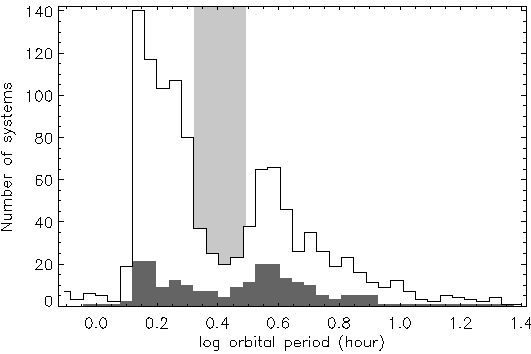
\includegraphics[width=\columnwidth]{figures/introduction/pd-rk.pdf}
    \caption{Reproduced from \citet{southworth2015}, Figure~14. The orbital period distribution of RKCat \citep{RKCat} CVs identified by the SDSS ({\bf white histogram}) and of the subset of these which are eclipsing ({\bf grey histogram}). The {\bf light grey shaded region} illustrates the period gap at 2.1 - 3.1 hours. The periods have been collected into histogram bins which are of equal size in log space.}
    \label{fig:period hist}
\end{figure}

The orbital period of a CV can be measured by tracking either their spectroscopic radial velocities (e.g. \citealt{gaensicke2009}), or the timings of repeating features in their lightcurves (e.g. \citealt{Littlefair2008}). Once this has been done for a large enough sample \citep{southworth2015}, a histogram of the periods can be plotted. This plot, shown in fig.~\ref{fig:period hist}, has three immediately obvious features:
\begin{itemize}
    \item a long period cutoff, as the number of systems taper off after $\sim12$hrs
    \item a period gap at $\sim2-3$hrs
    \item a period minimum at $\sim1$ hour, with a pile-up of systems just above it.
\end{itemize}
Each of these features are discussed in turn.

\subsubsection{The period maximum}
\label{sect:introduction:period maximum}
In order for a system be be a CV, mass must be transferring from a less massive star, onto a compact object, constraining the maximum value of $q$ to $\sim1$, and demanding that the secondary extends out to $\sim R_L$.

There are three constraints on a CV pertinent to the maximum allowable period. The mass ratio, $q = \frac{M_{\rm donor}}{M_{\rm WD}}$, must be low enough for thermally stable mass transfer ($q < 1.23$, \S\ref{sect:introduction:stability criterion}, here approximated as $q = 1.0$), the donor radius must be approximately equal to the Roche radius, and maximum mass of a white dwarf is well known to be limited to $\le 1.4M_{\odot}$ before triggering thermonuclear runaway \citep{chandrasekhar1942}.

Now, to find the theoretical period maximum, we simply find the period corresponding to the largest possible donor star. \citet{warner1995} shows that the average density, $\rho_{av}$, for objects that fill their $R_L$ follows a robust relationship;
\begin{equation}
    \frac{\rho_{av}}{\rho_{\odot}} = 75.9 P_{orb}^{-2}(h)
\end{equation}
\citet{knigge11} derived a connection between CV secondary mass and radius, $M_2$ \& $R_L$. This can be manipulated to produce a mass-period relationship,
\begin{align}
    \rho_{av} = \frac{3 M_2}{4 \pi R_L^3} &\simeq 75.9 P(h)^{-2} \\
    \frac{R_L}{R_\odot} = C &\cdot \Big( \frac{M_2}{D \cdot M_\odot} \Big) ^{\alpha}
\end{align}
where $C$ and $D$ are constants for a particular regime, i.e., short-period, long-period, or period bouncer, and $\alpha$ is the mass-radius index \citep{Knigge2011b}.
Combining the above gives a pleasingly simple relationship.
\begin{equation}
\label{eqn:MP_relation}
    M_2^{(1-3\alpha)} \propto P^{-2}
\end{equation}

For long-period CVs, $\alpha = 0.67\pm0.04$ \citep{knigge11}, and equation \ref{eqn:MP_relation} becomes $M_2^{1.01} \propto P^{2}$, and larger secondary masses require longer periods. The theoretical maximum secondary mass of $1.4 M_{\odot}$ corresponds to a period of $\sim12$hrs, though in reality these higher mass donors are rarer and the frequency of CVs at these higher periods begins to drop much earlier, at $\sim6$hrs \citep{gaensicke2009}.


\subsubsection{The period gap}
\label{sect:introduction:period gap}

Between periods of around 2-3 hours, there is a dramatic fall in the number of CVs we detect and volume-limited samples indicate that this is a real effect and not a selection bias \citep{Kolb1998,pala2020}. The origin of this gap in the period distribution is something of an open problem.

Models indicate that long period systems ($P > 3$h) have far higher mass loss rates than short period systems ($P < 2$h) \citep{ritter1985}. This suggests a significant change in braking mechanisms between the two regimes.
Recall that the donor star is inflated by mass loss (\S\ref{sect:introduction:Summary of how AML and Mdot drive period evolution}).
If the cutoff of angular momentum loss is sharp, i.e. magnetic braking suddenly ceases, the donor is allowed to contract to its equilibrium radius and disconnects from its Roche lobe, shutting off mass transfer.
The system is still subject to gravitational radiation, however, so gradually continues to evolve towards shorter periods. Once the secondary reconnects with its Roche lobe, mass transfer resumes and the system again presents itself as a CV, emerging from the period gap at a $\sim2$hr period \citep{kolb2002}.

The disruption of magnetic braking was proposed early on to explain the period gap \citep{rappaport1983, spruit1983}, and relatively shortly after \citet{kolb1993} showed more quantitatively that a sub-class of purely gravitational braking CV systems does not reproduce the observed population.
The classical evolutionary path of CVs has involved the secondary becoming fully convective which was thought to disrupt the magnetic field and so cease magnetic braking \citep{knigge11}.
\citet{Davis2008} used population synthesis to demonstrate that, if the period gap is caused by disrupted magnetic braking, this may affect the mass function of quiescent CVs that are moving through the gap. They expect an excess of non-transferring CVs over low mass post-common envelope CVs that emerge from the common envelope phase directly into the period gap.
These should form at a predictable rate across $q$, but due to the slow crossing of quiescent CVs the latter `pile up' in the gap - a detectable effect observed by \citet{zorotovic2011}.


\subsubsection{The period minimum, and period bouncer systems}
\label{sect:introduction:period minimum and bouncers}

The period minimum was first predicted by \citet{rappaport1982}, and can be understood by considering the two governing timescales affecting the secondary.
For donors with masses above $\sim0.1 M_{\odot}$, the donor is contracting in response to mass loss.
As this proceeds, both the Kelvin-Helmholtz (a.k.a. thermal) timescale, $\tau_{\rm KH}$, and mass transfer timescale, $\tau_{\dot M}$, are increasing (the latter due to $\dot M_2 / M_2$ rising as the period shrinks). However, $\tau_{\rm KH}$ rises faster, and at a period of $\sim80$ minutes \citep{ritter1998, McAllister2019}, $\tau_{\rm KH}$ exceeds $\tau_{\dot M}$, causing the donor to lose mass adiabatically and expand rather than contract in response to mass loss.
This allows the donor to remain in contact with its Roche Lobe when mass loss raises it to a higher orbit, and the system evolves to longer periods over time.

More quantitatively, as the components of a short period CV move closer together and the donor falls in mass, $\tau_{\rm KH}$ and $\tau_{\dot M}$ become more out of balance, corresponding to $\alpha$ in equation \ref{eqn:MP_relation} decreasing \citep{Knigge2011b}. A main-sequence star will have $\alpha \sim 1$, but a secondary subjected to fast, adiabatic mass loss will have $\alpha \simeq -1/3$. Looking at the gradient of equation \ref{eqn:MP_relation}, the existence of a period minimum can be easily seen.
\begin{equation}
    \frac{\dot P}{P} = \frac{(3\alpha - 1)}{2} \frac{\dot M_2}{M_2}
\end{equation}
When $\alpha \le 1/3$, a negative $\dot M$ will produce a \textit{positive} change in $P$, and the donor begins to retreat from the white dwarf \citep{rezzolla2001}.

This has been confirmed by \citet{knigge11}, who found that for period bouncer CVs, $\alpha = 0.21^{+0.05}_{-0.10}$, giving the following empirical version of equation \ref{eqn:MP_relation} in the post-period minimum regime.
\begin{align}
    M_2 \propto P^{-5.4}
\end{align}


\subsection{Problems with the classical picture}
\label{sect:introduction:modern AML}

A solid knowledge of exactly how and why CVs lose angular momentum has remained surprisingly elusive for several decades now. Early theories established gravitational waves and magnetic braking as the two main sources of AML, but attempts to quantify this with evolutionary models and population synthesis models consistently fall short. Gravitational losses are well understood, and have been independantly observed and studied, but the sources and consequences of magnetic braking is not so easy.

% The spin rates and masses of CV donors are not seen in the singleton stars that are usually used to characterise magnetic braking \citep{rappaport1983,matt2015,garraffo2018a}.
% In addition, the disruption of magnetic braking is often motivated by the donor transitioning to a fully convective state, but X-ray emission level is a diagnostic of magnetic flux \citep{pevtsov2003}, and \citet{wright2016} found that the X-ray flux of main sequence stars is similar between fully convective and non-convective main-sequence stars, implying a similar magnetic field strength. Furthermore, disagreement between observational and theoretical period gap and minimum locations \citep{knigge11} has left the disrupted magnetic braking model an area of active research.
% \citet{garraffo2018b} recently proposed that the magnetic field does not weaken, but rather becomes more complex which reduces the efficiency of magnetic braking. This concept is discussed quantitatively in \S\ref{sect:introduction:Garraffo magnetic braking prescription}.


\subsection{The missing AML problem}
\label{sect:introduction:the missing aml problem}

The evolution of CVs is driven by the donor stars. The orbital period is determined by the mass-radius relationship of the donor under mass loss, and the decay of the orbit should simply result directly from the two braking mechanisms (gravitational and magnetic). Figure~\ref{fig:introduction:Knigge 2011 figure 9} shows the relationship between the donor mass and orbital period, and the single unified CV track can be seen in the observations. CV evolution models can be built to try and reproduce this track, and indeed at long periods, our understanding of those mechanisms seem robust enough to produce models that satisfy observations. The period gap can, with some manual tweaks, also be reproduced with some accuracy. Unfortunately, at short periods ($\lesssim 2$ hours), the data begin to diverge from models \citep{knigge2006,knigge11}.

Section \ref{sect:introduction:Summary of how AML and Mdot drive period evolution} describes how the donor's mass-radius relation is altered by the presence of continued mass loss. The donor is larger than a singleton of the same mass, as the mass loss timescale is comparable to the thermal timescale and the donor is not quite able to maintain thermal equilibrium \citep{knigge11}. The degree of this inflation increases with more rapid mass loss. As mass loss is driven by AML, it follows that a CV donor that has stronger AML will have a larger radius, and therefore sit at a longer period than a CV with weaker AML, altering the gradient of the tracks in Figure~\ref{fig:introduction:Knigge 2011 figure 9} at periods of $\lesssim 3$ hours. In this way, the shape of the tracks in Figure~\ref{fig:introduction:Knigge 2011 figure 9} is a diagnostic of the form of AML experienced by a CV across its lifetime \citep{knigge11}.

\citet{knigge11} used observations of donor masses and radii and attempted to recreate the donor evolutionary sequence.
An unknown additional source of AML was added to their models, simply scaled relative to gravitational braking. This unknown contribution to AML is motivated by the disagreement between data and the model that omits this source. \citet{knigge11} find that the best-fit model to their data uses an excess braking below the period gap that is $2.47 \times \dot J_{GR}$, where $\dot J_{GR}$ is the AML due to gravitational waves. Figure~\ref{fig:introduction:Knigge 2011 figure 9} is reproduced from their work, and shows the significant improvement in agreement with data.
\begin{figure}
    \centering
    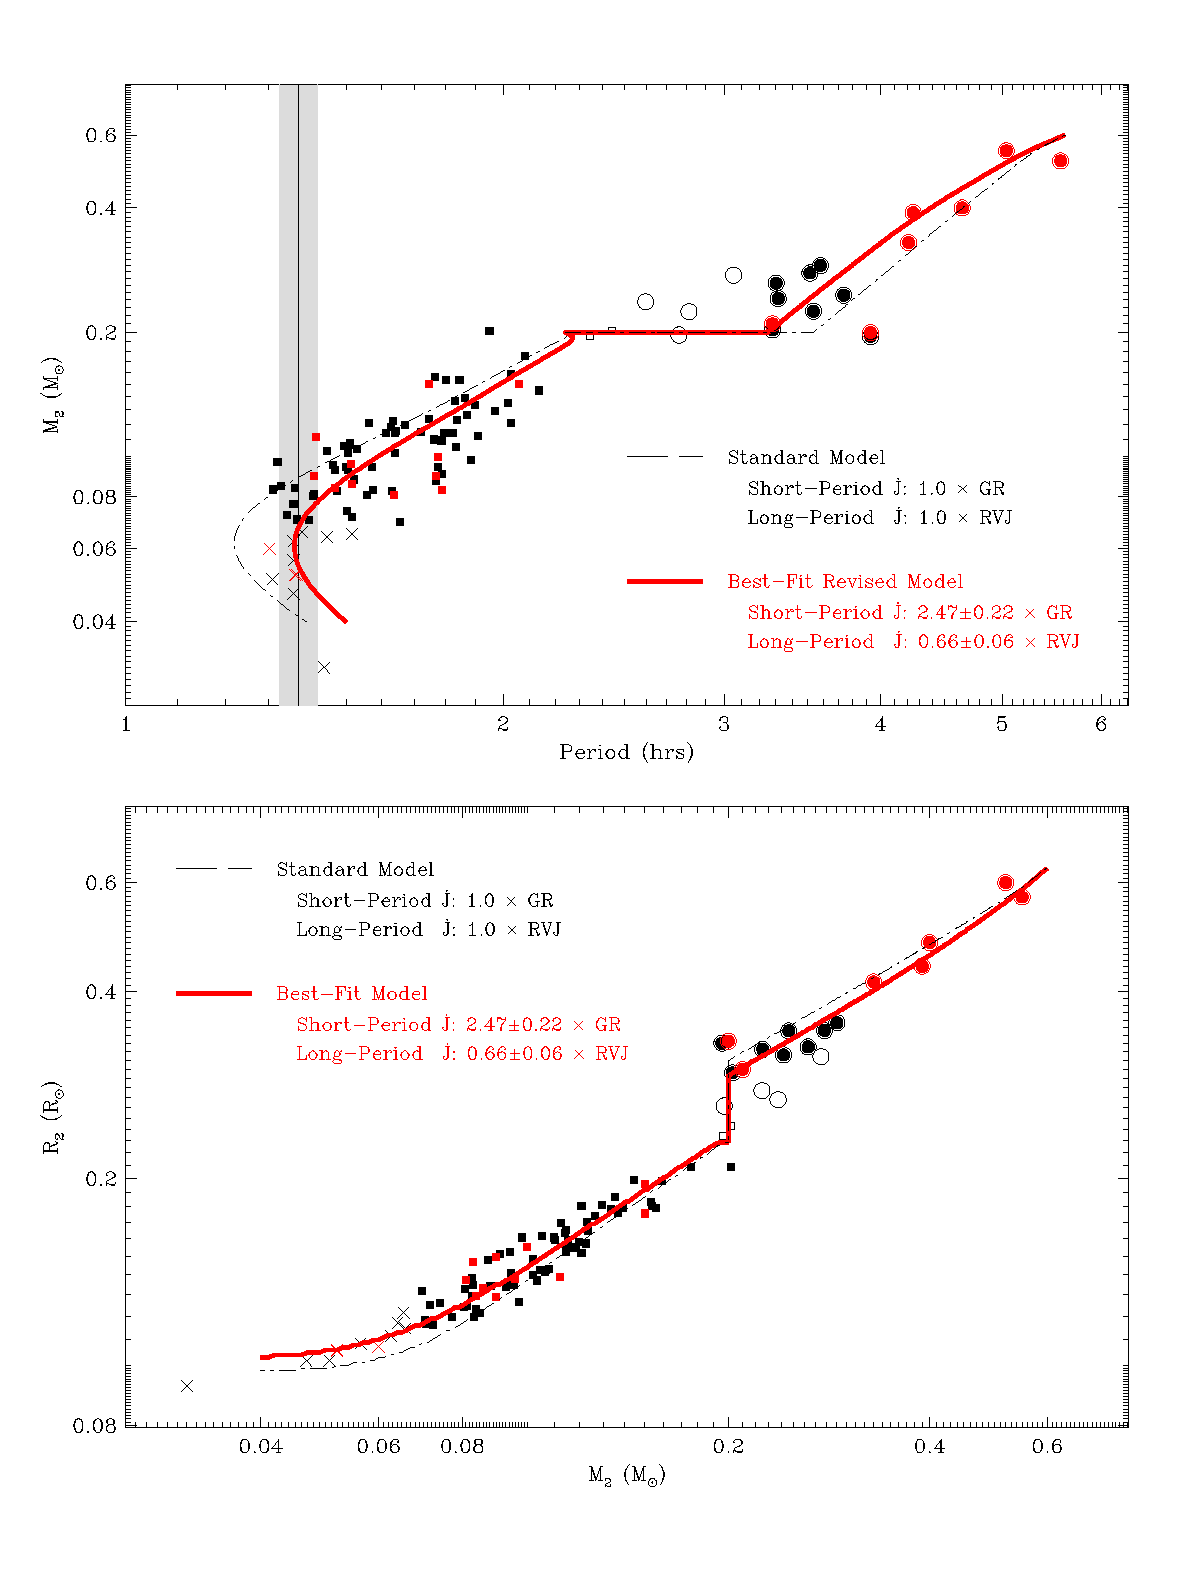
\includegraphics[width=\textwidth, trim={0 2cm 0 2cm}]{figures/introduction/Knigge11_fig9.pdf}
    \caption{Reproduced from \citet{knigge11}. {\bf Black} markers are data from superhumpers, {\bf Red} markers are data from eclipsers. {\bf Crosses} denote candidate period bouncer CVs, {\bf Squares} are short-period CVs, and {\bf Circles} are long period CVs. {\bf Open symbols} are omitted from their analysis due to lying in the period gap. The {\bf Dashed Black lines} are their `standard', na\"ive model, and the {\bf Solid Red line} includes an empirically determined excess AML source, scaled to gravitational wave braking. In the top panel, the {\bf Vertical black line} signifies the observed period minimum, with the grey region as the FWHM of the period spike as measured in \citet{gaensicke2009}.}
    \label{fig:introduction:Knigge 2011 figure 9}
\end{figure}

\citet{Pala2017a} used the effective temperatures of the white dwarfs to probe CV evolution. The white dwarf temperature can be enhanced by accretion, so a hotter white dwarf suggests a higher mass transfer rate. This is sensitive to changes in $\dot M$ on relatively short timescales ($\sim 10^4$ yrs), but still provides a valuable insight. \citet{Pala2017a} compare their white dwarf temperatures (and therefore mass transfer rates, and therefore AML rates) to MESA CV evolutionary tracks, and find that their observed temperatures are poorly described by only gravitational AML, but are more well-fitted by models that includes excess AML equivalent to gravitational losses, i.e. double-strength gravitational AML.

The disagreement between theory and observation at short periods indicates that our understanding of AML in this regime is lacking, and a few proposals to rectify this have been suggested.

The obvious solution to the problem of missing AML is that we simply do not understand magnetic braking well enough to say that it fully disappears below the period gap. The donor may retain a residual magnetic field strong enough to drive some weaker form of magnetic braking that remains after the bulk of magnetic braking ceases, a.k.a. residual magnetic braking.

The period gap is frequently attributed to a fall in magnetic braking when the donor becomes fully convective, due to a large reduction in magnetic field strength. However, observations of field M dwarfs of similar masses, with convective envelopes, are seen with key tracers of magnetism. Specifically, X-ray observations find that the coronal magnetic energy dissipation of fully convective stars is similar to non-convective stars \citep{wright2016}, and Zeeman-Doppler imaging of rapidly rotating M dwarfs indicate that magnetic fields remain strong, whilst the complexity of surface magnetic fields increases alongside rotation rate (e.g. \citealt{donati2003,donati2009,marsden2011,waite2011,waite2015}).
Together, these observations strongly indicate that the disrupted magnetic braking model commonly accepted is ill-motivated, and may be more closely tied to field complexity than field strength \citep{garraffo2018b}. If the gap is indeed driven by a sudden increase in field complexity, then it is reasonable to assume that magnetic braking may remain significant after the system emerges from the period gap.

% Additionally, the whilst magnetic braking is obviously not possible with too weak a magnetic field, it is also not possible under magnetism that is too strong. Some evidence for AML suppression under strong magnetic fields, though not in the context of the period gap, has been found in binary population synthesis models that focus on magnetic CVs \citep{belloni2020}. The models that include magnetic wind suppression under a strong white dwarf magnetic field result in a better fit to key CV observables -- specifically the orbital period distribution, white dwarf temperature distribution, and space density.

Magnetic braking is not the only possible explanation for excess AML, and another strong candidate is consequential AML. This mechanism is discussed below.


\subsection{Consequential AML}
\label{sect:introduction:CAML}

Consequential AML (CAML) is an additional source of momentum loss, originally motivated physically as a second source of magnetic wind emanating from the inner regions of the white dwarf accretion disc \citep{king1995,schenker1998}. In more modern considerations of CAML, the excess loss is explained as nova events temporarily immersing the system in a viscous medium, causing drag on the two bodies and reducing their orbital separation \citep{Schreiber2016}.
In each case, this AML is ``consequential'', in the sense that they rely on either a pre-existing disc to be present or the white dwarf to be accreting enough mass to trigger novae, and the CAML disappears in the absence of existing AML.
By modelling CV evolution including this process, several issues of older CV population synthesis and evolutionary models can be solved at once \citep{Schreiber2016}. These issues are:
\begin{enumerate}
    \item the observed mass of CV white dwarfs is systematically higher than singleton white dwarfs (e.g. \citealt{McAllister2019,pala2020});
    \item since the short period regime has much lower AML rates, CVs should spend most of their time below the period gap, and $\sim 99\%$ of CVs are expected to be short period \citep{kolb1993a}, but observations see a less severe imbalance between long (17\%) and short (83\%) period systems \citep{pala2020};
    % roughly even distribution between long and short period systems \citep{knigge2006};
    \item under purely gravitational losses, the period minimum was first calculated at $\sim 67$ minutes \citep{kolb99}, but is observed at $\sim 79$ minutes \citep{McAllister2019};
    \item the space density of CVs is roughly 1-2 orders of magnitude lower than population synthesis models predict.
\end{enumerate}
The introduction of a modified, empirically calibrated CAML produces models that do not suffer from these issues, making a compelling case for its validity.

The maximum dynamically stable mass transfer rate of a CV is a function of $q$, related via the adiabatic mass-radius exponent, $\xi_{ad}$, and the mass-radius exponent of the Roche radius, $\xi_{L}$. Where the two intersect forms a threshold beyond which runaway mass transfer (much like the pre-CV common envelope phase) is triggered, and most likely results in a merger between the two bodies. We begin similarly to the derivation in \S\ref{sect:introduction:stability criterion},
\begin{equation}
    \label{eqn:introduction:CAML stability threshold}
    \xi_{ad} = \frac{{\rm d} ln(R_2)}{{\rm d} ln(M_2)}_{ad} = \frac{{\rm d} ln(R_L)}{{\rm d} ln(M_2)} = \xi_L
\end{equation}
where $\xi_{ad}$ for convective stars is $-1/3$. Recalling the Eggleton approximation for the Roche radius, Equation~\ref{eqn:introduction:eggleton approximation}, we can find $\xi_{ad}(q)$ \citep{Schreiber2016} in the absence of CAML,
\begin{equation}
    \xi_{ad} = \frac{2}{3}\frac{ln(1+q^{1/3}) - \frac{1}{2}\frac{q^{1/3}}{1+q^{1/3}}}{0.6q^{2/3} + ln(1+q^{1/3})} (1 + q) + 2(q - 1) = -1/3
\end{equation}
Solving this equation gives a critical maximum value of $q \lesssim 0.634$. However, under CAML, extra sources of $\dot J$ are introduced. For example, under the classical non-conservative construction, $\dot J_{CAML}$ is due to nova ejecta carrying angular momentum away from the system as it leaves, contributing
\begin{equation}
    \frac{\dot J_{CAML}}{J} = \nu \frac{\dot M_2}{M_2}
\end{equation}
Here, $\nu = M_2^2 / (M_1(M_1 + M_2))$ and encapsulates the assumption that the angular momentum carried by ejected nova material is equal angular momentum to the white dwarf.
The right hand side of Equation~\ref{eqn:introduction:CAML stability threshold} is then altered by the increased AML rate.
\begin{equation}
    \xi_{ad} = \frac{2}{3} \Bigg( \frac{ln(1+q^{1/3}) - \frac{1}{2}\frac{q^{1/3}}{1+q^{1/3}}}{0.6q^{2/3} + ln(1+q^{1/3})} \Bigg) + 2\nu + \frac{M_2}{M_1 + M_2} - 2
\end{equation}
The effect of this altered form of $\xi_{ad}$ is that CVs with higher mass ratios are stable. Binary population synthesis models by \citet{Schreiber2016} demonstrate that this model is not compatible with observations, producing {\it more} CVs with low mass donors than the non-CAML model and actually performing worse than models that don't include this version of CAML. However, by altering the form of $\nu$ so that it is no longer tied to the white dwarf's angular momentum, a much better agreement with observations can be reached. This is the empirical CAML model, or eCAML.

$\nu$ is altered to a simple function of the white dwarf primary mass,
\begin{equation}
    \label{eqn:introduction:eCAML nu}
    \nu ( M_1 ) = \frac{C}{ M_1 }
\end{equation}
where $C$ is an arbitrary constant chosen to best reflect observations, and \citep{Schreiber2016} adopt values of $C = 0.3 - 0.4$.
The inverse relationship of more CAML at lower white dwarf masses is motivated by lower mass systems ejecting nova material at a lower velocity, meaning the binary is immersed in a friction-generating medium for longer and imparting more energy into the ejecta.

With eCAML, the dynamically unstable region is expanded. This has the important effect of making CVs with low-mass white dwarfs prone to dynamically unstable mass transfer (see \S\ref{sect:introduction:stability criterion}), removing them from the CV population -- this simultaneously answers the question of CV white dwarfs being more massive than expected, and also vastly lowers the space density \citep{belloni2018}. Finally, the majority of systems that are now dynamically unstable are short-period CVs, so the observed period distribution is significantly more well-reproduced. Figure~\ref{fig:introduction:Schreiber 2016 figure 2} is reproduced from \citet{Schreiber2016}, and shows the three dynamically unstable regions graphically.
\begin{figure}
    \centering
    \begin{minipage}[b]{\textwidth}
        \centering
        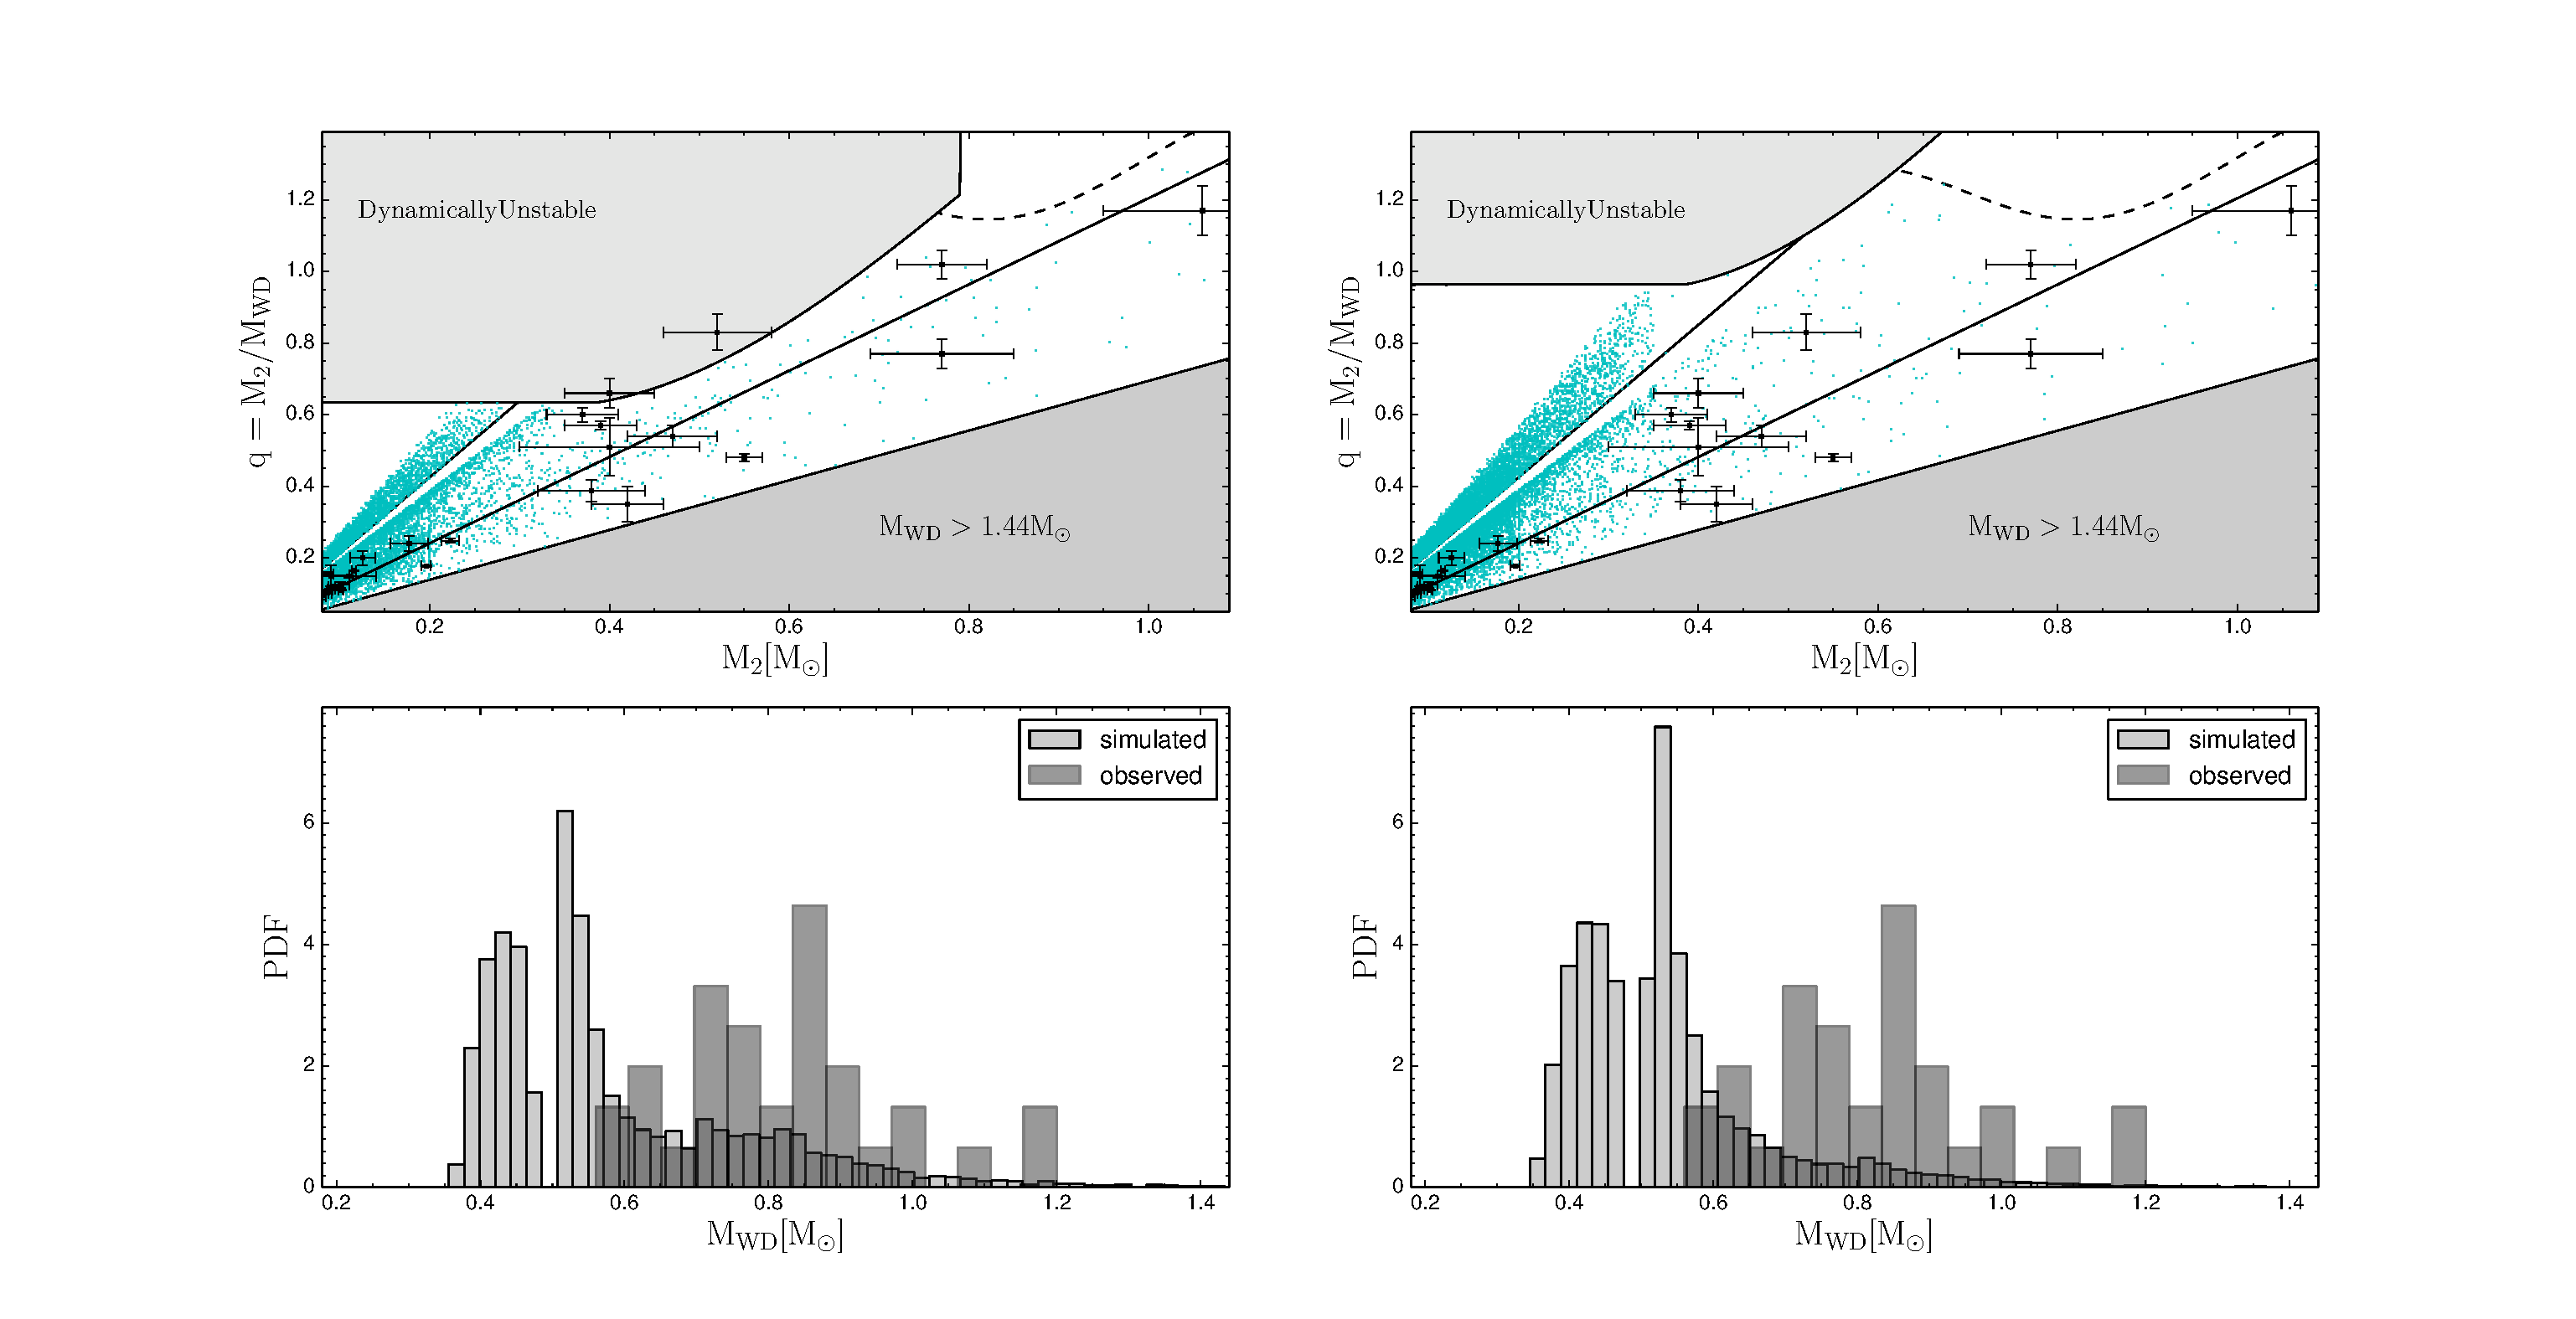
\includegraphics[width=0.8\textwidth,trim={22cm 12cm 0 0},clip]{figures/introduction/Schrieber_figure1.pdf}
    \end{minipage}
    \begin{minipage}[b]{\textwidth}
        \centering
        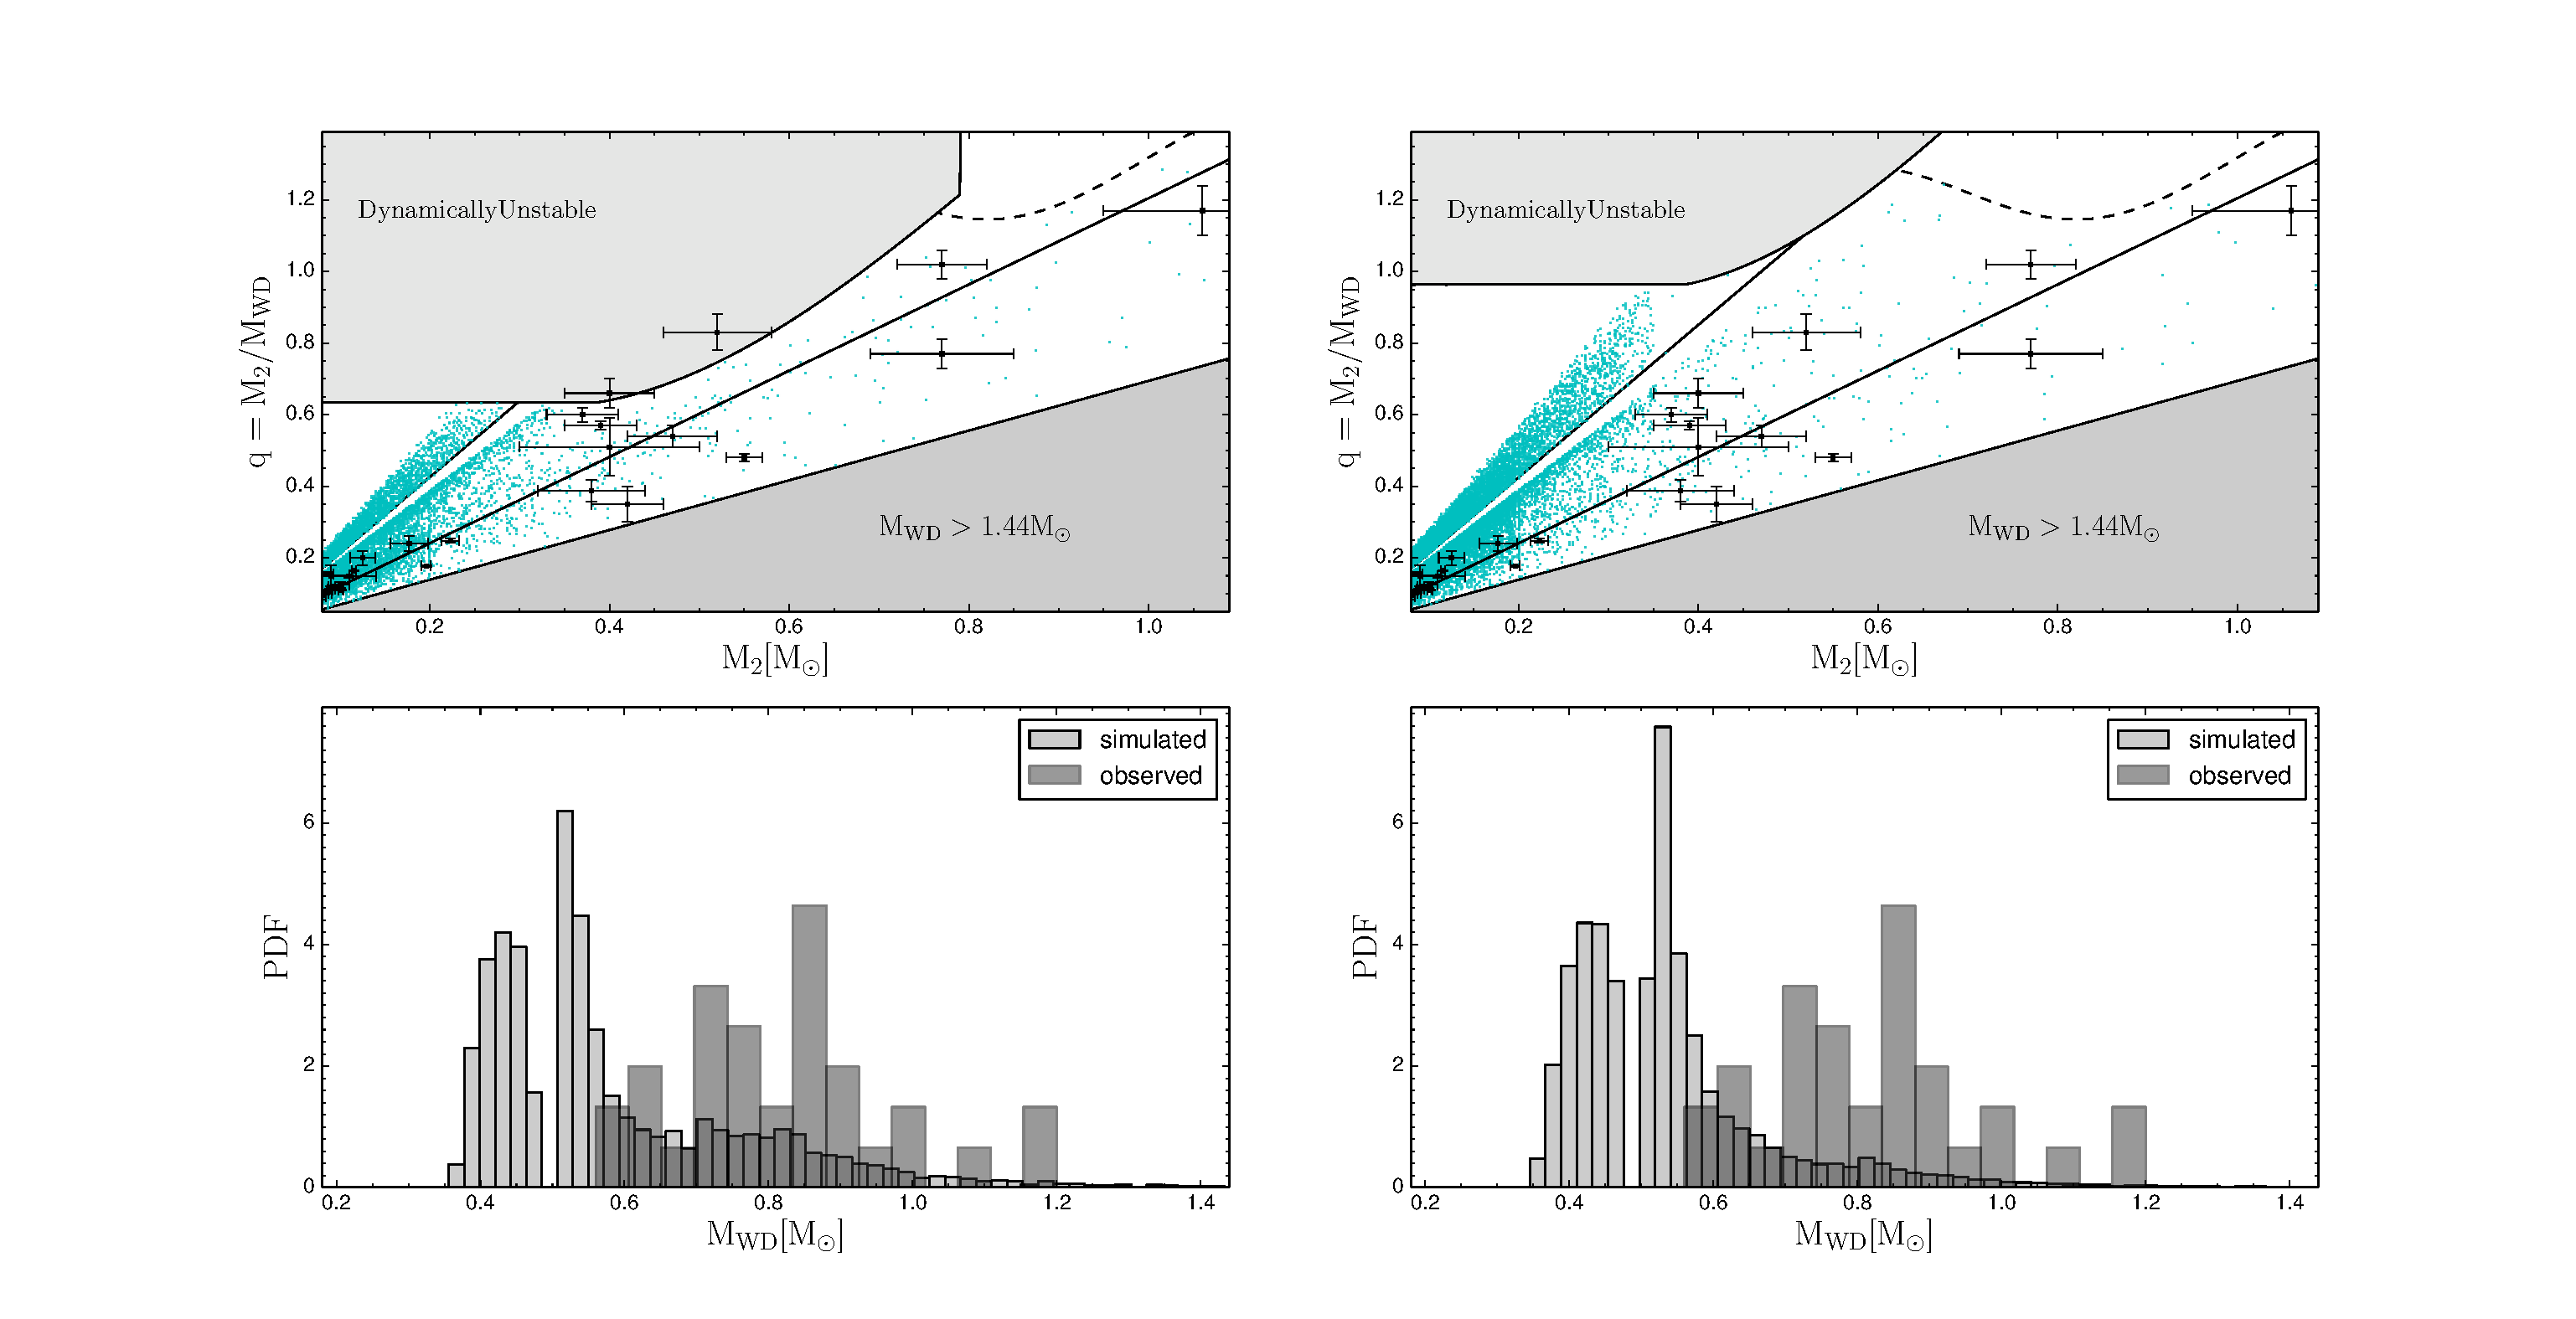
\includegraphics[width=0.8\textwidth,trim={0 12cm 22cm 0},clip]{figures/introduction/Schrieber_figure1.pdf}
    \end{minipage}
    \begin{minipage}[b]{\textwidth}
        \centering
        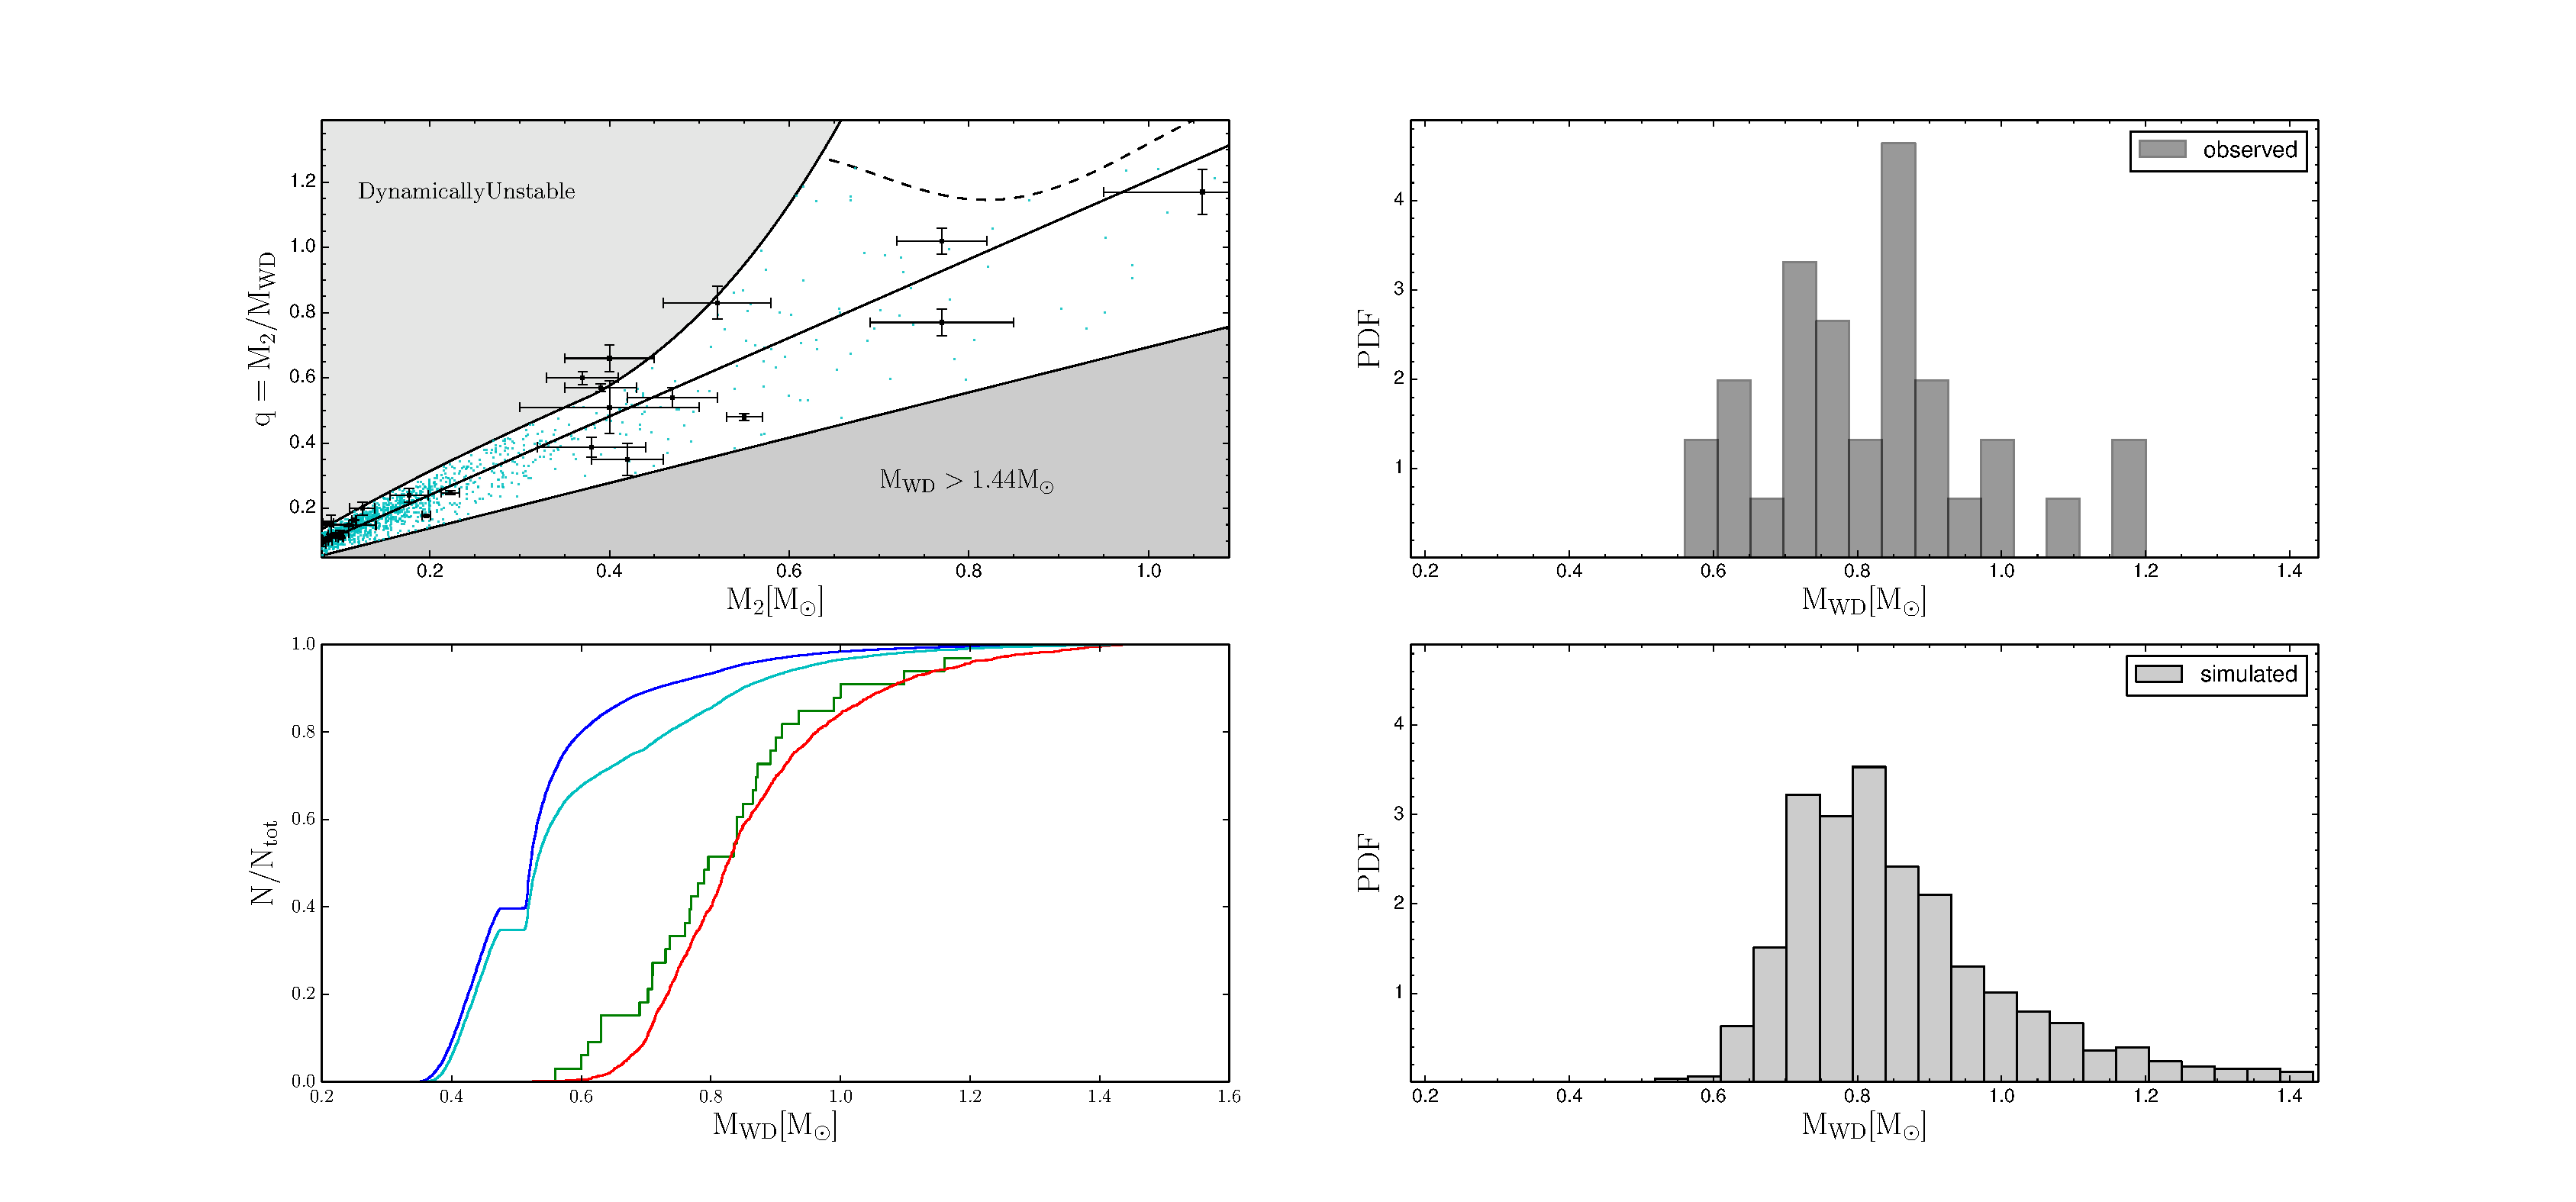
\includegraphics[width=0.8\textwidth,trim={0 12cm 24cm 0},clip]{figures/introduction/Schrieber_figure2.pdf}
    \end{minipage}
    \caption{Reproduced from Figure~2 and Figure~3 of \citet{Schreiber2016}. {\bf Black squares} are observed CVs, and {\bf cyan dots} are predicted CV populations. {\it Top} is for a fully conservative CV model, the {\it middle panel} is for the classical non-conservative model, and the {\bf bottom panel} is the eCAML results. The $M_{WD} > 1.44 M_\odot$ regions are forbidden, as these white dwarfs exceed the Chandrasekhar limit.}
    \label{fig:introduction:Schreiber 2016 figure 2}
\end{figure}

Some observational evidence for eCAML has recently been uncovered by \citet{Pala2021}, where an inverse correlation between white dwarf mass and mass loss rate was observed. This is in line with Equation~\ref{eqn:introduction:eCAML nu}.
Also, low mass ($<~0.5M_\odot$) helium-core white dwarfs are expected to be formed in binaries, but are frequently observed as singletons. The merger scenario under eCAML provides a neat explanation for this \citep{zorotovic2017}.
In addition, \citet{sparks2021} observed the spectra of CV donors and found significant non-solar abundances,  indicating that after nova outbursts, some of the nova-processed material is retained in the system long enough to be accreted onto the donor, and is supportive both of lower mass white dwarfs having a lower eCAML contribution, and of the donor being immersed in nova material long enough to accrete significant amounts of it.


\subsection{Magnetic Braking}
\label{sect:introduction:magnetic braking}

The M dwarf secondary of a CV will emanate some wind, made up of charged ions, and have some magnetic field which co-rotates with the star.
Consider a blob of charged wind material, moving with some sideways velocity in the plane of the orbit, almost certainly slower than the magnetic field lines.
The blob will interact with the field and be accelerated to co-rotate with them.
This higher velocity causes it to move outwards, to a higher orbit, where the field lines are moving even faster, accelerating the blob more.
As the wind material is accelerated, it exerts a drag force on the magnetic field of the donor and slows its rotation rate.
The close proximity of the binary means that tidal effects are strong, and the donor is spun up again by robbing the orbit of angular momentum, reducing the binary separation and hardening the binary \citep{verbunt1981}.

As an aside, \citet{wickramasinghe1996} presented theoretical motivation that the white dwarfs in CVs can have too strong a magnetic field to allow magnetic braking. Open field lines are necessary for wind to escape the system, so too strong a white dwarf magnetic field can trap the ionised gas in-system, suppressing the wind of the secondary.
Evidence for AML suppression under strong magnetic fields has been found in binary population synthesis models that focus on magnetic CVs \citep{belloni2020}. The models that include magnetic wind suppression under a strong white dwarf magnetic field result in a better fit to key CV observables -- specifically the orbital period distribution, white dwarf temperature distribution, and space density.

When building a magnetic braking model, assumptions must be made about the effects of the magnetic field strength and field geometry, as well as how the wind speed scales with the donor's mass, radius, and rotation rate. The adopted values for these free parameters are tuned to match open cluster data, as open clusters can have their ages determined, and the masses, radii, and rotation rates of the stars contained in them observed (e.g. \citealt{matt2015,garraffo2018a}). The CV community is able to use these findings to inform CV models.
However, the parameter space covered by open cluster data does not cover the parameter space occupied by CVs. Rotation rate is a key variable in magnetic braking prescriptions, but the typical CV rotational period is on the order of a few hours, and singleton M dwarfs are considered extremely fast rotators with periods of a day -- a difference of an order of magnitude. Observations of singletons simply do not reach to the extremely low mass, rapid rotations that are frequently seen in CVs, so we are forced to rely on extrapolation and theory.

This carries with it some major practical issues. One is that whilst the broad effects of magnetic fields is relatively easy to intuit, quantitative physical understanding the mechanics and origins of magnetic fields is difficult, involving fluid dynamics, considering interactions with the accretion disc, and magnetism acting on large systems, which quickly become prohibitive to model and is usually handled with one of a variety of recipes. \citealt{knigge11} contains a detailed compilation of some older approaches, but the decade since has seen a few newer methodologies emerge. Here, two recent magnetic braking prescriptions are described in moderate detail: the \citet{matt2015} prescription, and the \citet{garraffo2018a} prescription. For a more complete, detailed summary of the modern understanding of M dwarf magnetic fields refer to \citet{kochukhov2021}.


\subsubsection{Matt prescription for magnetic torque}
\label{sect:introduction:matt braking}

In \citet{matt2015}, an empirical prescription is derived that relates the torque felt by a low mass main sequence star to that stars' mass, radius, and Rossby number, $Ro$. $Ro$ is a fluid dynamics term for the ratio between the inertial and Coriolis force terms of the Navier-Stokes equations. A small $Ro$ indicates a system dominated by Coriolis effects, and a large $Ro$ indicates that centrifugal and inertial forces dominate. The $Ro$ of a main sequence star can be calculated from its rotation period, $P_{rot}$, and the convective turnover timescale, $\tau_{\rm cz}$.
\begin{equation}
    \label{eqn:introduction:rossby number}
    {Ro} = \frac{P_{rot}}{\tau_{\rm cz}}
\end{equation}
Through $Ro$, the effectiveness of magnetic braking is tied to rotation, which is extremely fast in CVs, and stellar mass and age, which affect $\tau_{\rm cz}$.

\citet{matt2015} make use of observations of stars with masses between $0.15 - 1.3 M_\odot$ and ages of $\sim 10^{6-9}$ yrs, that have had their rotation periods measured. This dataset is used to calibrate a theoretically motivated empirical prescription for magnetic braking. There is some evidence for a saturation of magnetic activity below a critical Rossby value (a.k.a. above a critical rotational period) \citep{reiners2009}, where magnetic activity seems to no longer respond to changes in rotation. \citet{matt2015} therefore adopt two relationships for torque, $T$, modulated by an empirical value, $p$,
\begin{equation}
    T = -T_0 \bigg( \frac{\tau_{\rm cz}}{\tau_{cz,\odot}} \bigg)^p \bigg( \frac{\Omega_{*}}{\Omega_{\odot}} \bigg)^{p+1}
\end{equation}
for the unsaturated regime, and
\begin{equation}
    T = -T_0 \chi^p \bigg( \frac{\Omega_*}{\Omega_\odot} \bigg)
\end{equation}
in the saturated regime. In both cases, $p$ is assigned as $p = 2$ in order to agree with the most common literature spin-scaling prescription, $T \propto \Omega_*^3$.
$\chi$ is the inverse critical $Ro$ for saturation, for which \citet{matt2015} adopt a value of $10$.
The rotation rates of the donor and the sun are $\Omega_{*,\odot}$ respectively, and $T_0$ is given by a function of mass and radius,
\begin{equation}
    T_0 = 9.5 \times 10^{30} {\rm erg} \bigg(\frac{R_*}{R_\odot} \bigg) \bigg(\frac{M_*}{M_\odot} \bigg)
\end{equation}

The authors take observations of two clusters, the $\sim 5$ Myr old ONC cluster and the $\sim 580$ Myr old Praesepe cluster, and use the first as initial conditions and the second as target distribution to reproduce. Figure~\ref{fig:introduction:Matt 2015 figure 2} is taken from \citet{matt2015}, and compares the initial and final conditions of their synthetic cluster model compared to these two boundary conditions. During the first few tens of Myrs of this model, the stars in the synthetic cluster are spun up as they contract, lowering their periods by factors of $\sim 5-10$. After this initial phase, which is much shorter than the spin down timescales, the more long-term spin evolution begins.
\begin{figure}
    \centering
    \begin{minipage}[b]{\textwidth}
        \centering
        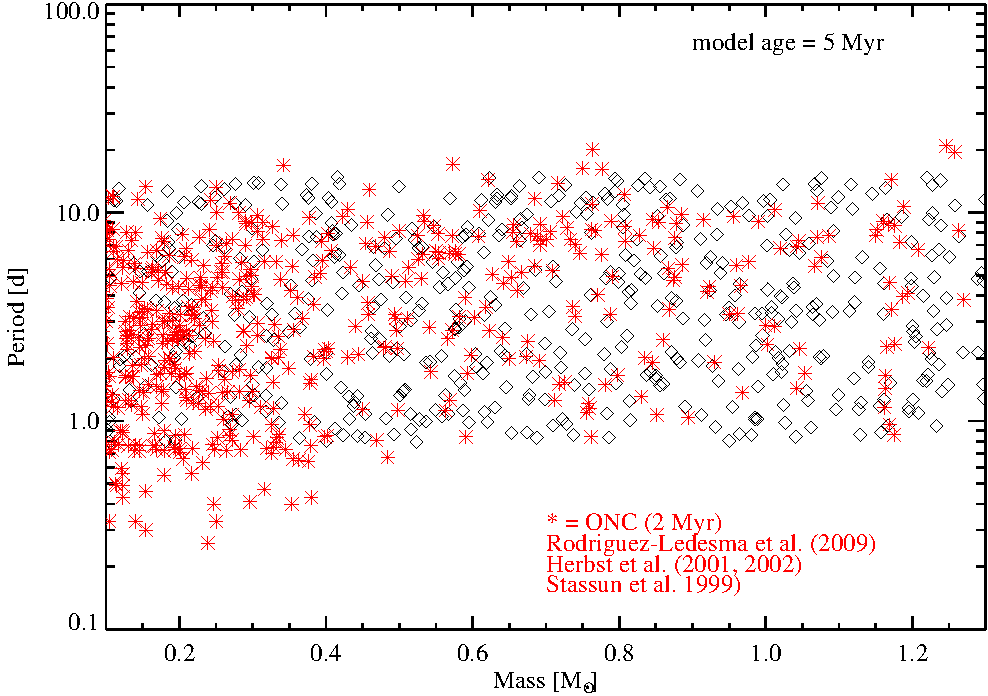
\includegraphics[width=0.8\textwidth]{figures/introduction/matt_2015_fig2a.pdf}
    \end{minipage}
    \begin{minipage}[b]{\textwidth}
        \centering
        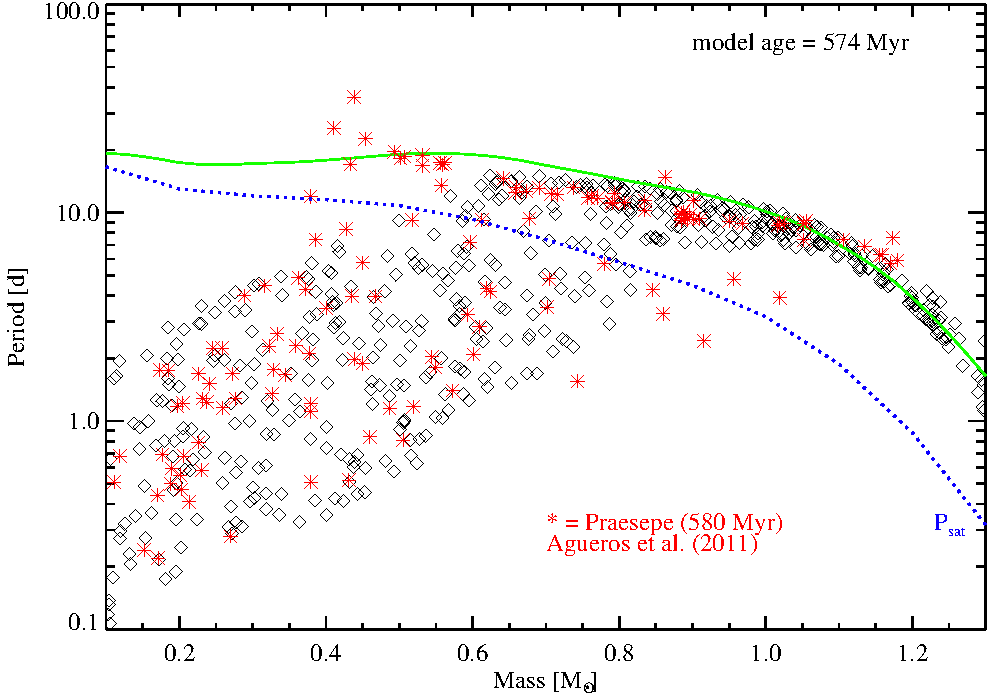
\includegraphics[width=0.8\textwidth]{figures/introduction/matt_2015_fig2b.pdf}
    \end{minipage}
    \caption{Figure taken from \citet{matt2015}. {\bf Red crosses} are observations of the ONC ({\it top}) and Praesepe ({\it bottom}) cluster stars. {\bf Black diamonds} are synthetic cluster stars. In the bottom panel, the {\bf solid green line} is the theoretical asymptotic spin rate of unsaturated stars and the {\bf dotted blue line} delimits magnetically saturated and unsaturated stars.}
    \label{fig:introduction:Matt 2015 figure 2}
\end{figure}

The agreement between the synthetic cluster and the Praesepe cluster at 574 Myrs is impressive. Above $\sim 0.8 M_\odot$, stars converge on a single narrow mass - period track just as is seen in the observations, and the large scatter below $\sim 0.8 M_\odot$ is also reproduced. Also, just as is seen in the cluster observations of Praesepe, the fastest rotators are those with the lowest masses. Both of these features arise from the transition from saturated braking, to unsaturated braking \citep{matt2015}.

At formation, almost all stars are experiencing saturated magnetic braking. The single narrow track arises from higher mass stars spinning down faster than lower mass stars, moving them off the much less efficient saturated braking regime sooner. The pile-up of systems then produces the narrow track. The mass dependancy of this track comes from the fact that spin-down timescale in the saturated regime is shorter for higher mass stars.
The broad population of low mass rapid rotators is a direct result of the broad initial conditions, which span an order of magnitude themselves, and the longer spin-down time of lower mass stars in the saturated regime allowing them to remain at high rotation rates for longer.

However, this model does fail in a few key respects. In the bottom panel of Figure~\ref{fig:introduction:Matt 2015 figure 2}, a small population of very slow rotators can be seen at $\sim 0.4 M_\odot$. The slower rotation rates of these stars suggests an alternative spin-down mechanism. The inverse problem is seen at $\sim 0.7 M_\odot$, where a handful of stars are seen rotating {\it faster} than predicted by any of the synthetic cluster stars, suggesting that magnetic braking is not as effective in their case.
More importantly for the CV field, the parameter space of CVs is completely uncovered, as CVs have rotation periods of $< 0.2$ days, and the systems that this work concerns have periods of $\lesssim 0.07$ days. Whilst this would firmly place CVs in the saturated regime, there is evidence of a `supersaturated' regime at extreme rotation periods that may be relevant to CV donors \citep{James2000, Wright2011, Argiroffi2016}. This possibility is also noted by \citet{Gossage2021} when outlining best practice use of this prescription in the stellar evolution code MESA, though the subject is not a settled matter and competing evidence for the {\it lack} of supersaturation has been reported by \citet{jeffries2011}.


\subsubsection{Garraffo prescription for magnetic torque}
\label{sect:introduction:Garraffo magnetic braking prescription}

The \citet{garraffo2018a} model considers the morphology of the magnetic field to also be important to the strength of magnetic braking, based on the work by \citet{garraffo2015}. The primary justification for this inclusion is observations of open clusters of a known age, where a bimodality is seen in the rotation rates of stars of similar masses. Some stars appear to be fast rotators, and some are slow rotators, and there is a dearth of systems between the two.
Previous attempts to model this bimodality have relied on an unexplained transition between an efficient braking state, and an inefficient braking state \citep{spada2011,reiners2012, gallet2013}, and \citet{garraffo2018a} expand on this by offering a shift in magnetic field morphology as the underlying trigger.

Their formalisation of this is based on two assumptions. They assume that stars with a dipolar magnetic field follow a known spin-down law, with a mass dependence reflecting $\tau_{\rm cz}$ \citep{skumanich1972}. Second, they assume that there is some relationship between field morphology and stellar spin rate. Specifically, that stars rotating more rapidly have more complex magnetic fields. This is formalised via an AML rate, $\dot J$,
\begin{equation}
    \dot J = \dot J_{\rm dipole}Q_J(n)
\end{equation}
where $\dot J_{\rm dipole}$ is the dipole loss under the Skumanich law, $\dot J_{\rm dipole} \propto \Omega^3 \tau_{\rm cz}$. $Q_J$ is a modulating factor that encapsulates the field complexity at the stellar surface, and is controlled by the complexity factor, $n$, which is a function of $Ro$. \citet{garraffo2016} derive an equation for $Q_J$, based on fitting the results of magneto-hydrodynamic simulations with varying field complexities.
\begin{equation}
    \label{eqn:introduction:garraffo complexity modulation}
    Q_J(n) = 4.05 e^{-1.4n} + \frac{n-1}{60Bn}
\end{equation}
Where $B$ is the magnetic field strength at the stellar surface. As the second term is only significant for $n > 7$, \citet{garraffo2018a} consider $n = 7$ as the maximum complexity, and consider only the first term of this relation. This is the equivalent of the saturation of magnetic braking, but here is contingent on field complexity rather than $Ro$.

\citet{garraffo2018a} suggest the following relation between $Ro$ and $n$,
\begin{equation}
    \label{eqn:introduction:garraffo field complexity}
    n = 1 + \frac{x}{Ro} + (y \cdot Ro)
\end{equation}
where $x$ and $y$ are free parameters, chosen to fit observations of open clusters. The three terms reflect three aspects of the magnetic braking model - the minimum complexity is defined as $n \equiv 1$, the first factor encodes stars with small $Ro$ having large $n$ (e.g. young, fast rotators), and the third term gives stars with large $Ro$ similarly large $n$ to explain the observed population of old rapid rotators that appear to have experienced minimal spin-down \citep{vanSaders2016}.
This prescription explains the AML of a star as purely a function of $Ro$.

Similarly to \citet{matt2015}, \citet{garraffo2018a} run a population synthesis model to compare to observations using initial conditions taken from the 13 Myr old h Persei cluster \citep{moraux2013}, but the authors show that differences between alternative initial conditions do not survive longer than 200 Myrs. Observations of stellar rotation periods and colour from several clusters with known ages are then compared to the synthetic population.

The resulting distribution does recover the Skumanich bifurcation observed in open clusters, reproducing the fast and slow rotating populations and the gap between them, though the large uncertainty in the age of the cluster does introduce some discrepancy.
In addition, the synthetic cluster does not consider the effects of close binary stars, which will affect the spin-down rate through tidal effects. However, this effect is ignored by the author, as there is evidence that the binary fraction in open clusters is low \citep{meibom2007}.
The mass dependency of this track is also reproduced by the model, and Figure~\ref{fig:introduction:garraffo 2018a fig 4}.
\begin{figure}
    \centering
    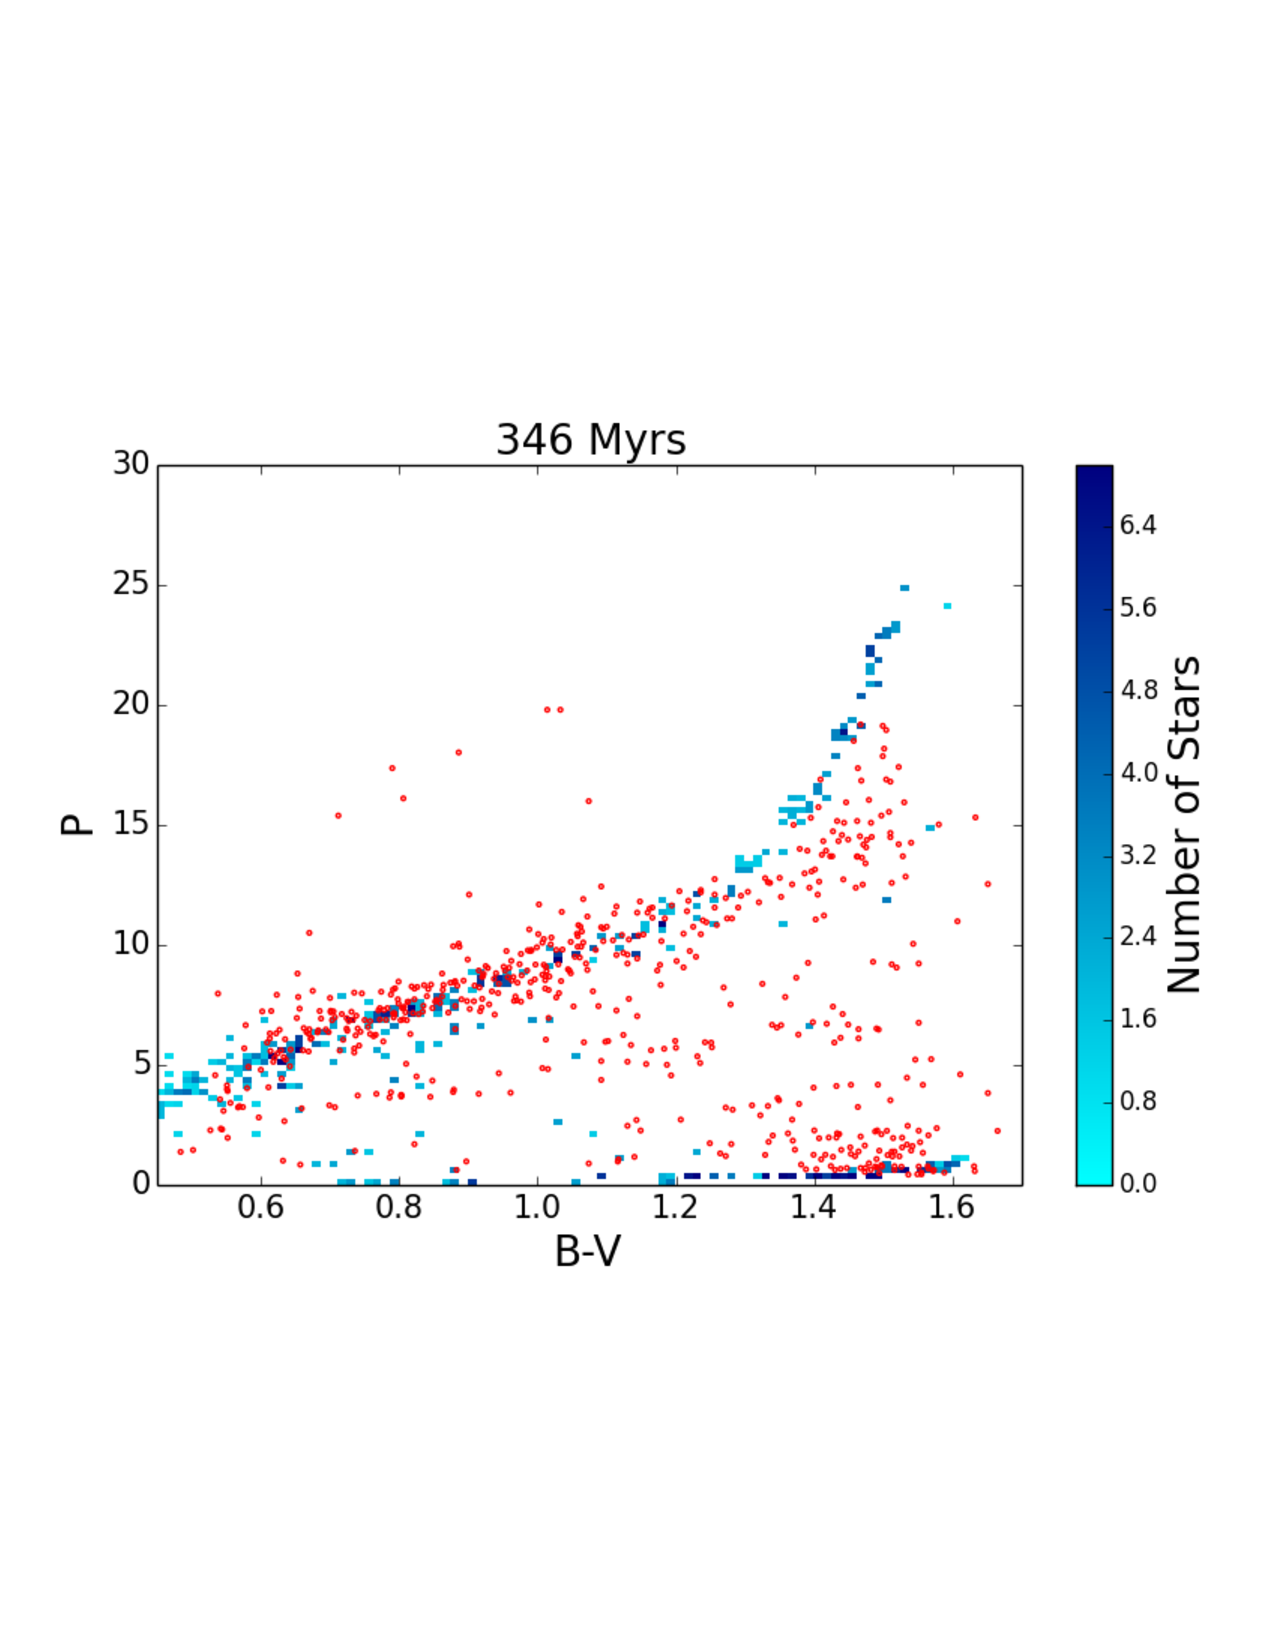
\includegraphics[width=0.7\textwidth, trim={0 5cm 0 5cm}]{figures/introduction/garraffo2018_M37_346_hPer.pdf}
    \caption{Example comparison between synthetic and observed cluster populations taken from \citet{garraffo2018a}. {\bf Red points} are observations of M37, which has its age measured at $\sim 346 - 550$ Myrs. {\bf Blue points} are the probability distribution of the synthetic cluster population from \citet{garraffo2018a}.}
    \label{fig:introduction:garraffo 2018a fig 4}
\end{figure}

The \citet{garraffo2018a} prescription is simpler in concept than the \citet{matt2015} prescription, and both prescriptions perform well. However, neither formulation covers the parameter space of CV donors, and both are semi-empirical with some arbitrary decisions made in order to fit open cluster data. This makes both approaches highly vulnerable to extrapolation errors and difficult to trust in the context of CV evolution, especially in the short period regime.


\subsubsection{Comparisons to the Rappaport, Verbundt and Joss model}

We can examine the differences between these prescriptions in the case of CV evolution by applying them to a donor evolutionary track, and \citet{knigge11} has constructed a donor sequence using their own models that reasonably accurately reproduces observations. The masses, radii, and periods along the sequence are given, so the would-be effects of the magnetic braking prescriptions described above can be calculated. In addition to the two previously discussed prescriptions, the default MESA \citep{Paxton_2015} magnetic braking prescription \citep{rappaport1983} is included. This prescription includes a magnetic braking index, $\gamma$,
\begin{equation}
    \dot J = -3.8\times10^{-30} M R_\odot^4 \bigg( \frac{R}{R_\odot} \bigg)^\gamma \omega^3\  {\rm dyn\ cm}
\end{equation}

Note that in the specific case of CVs, period and radius are synonymous with one another due to the requirement that the donor is in contact with the Roche lobe, and is tidally locked.

\begin{figure}
    \centering
    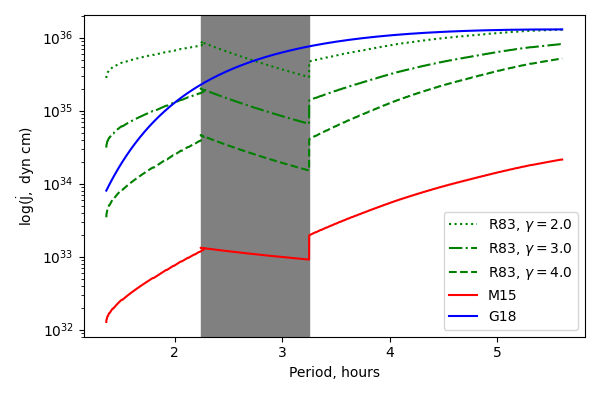
\includegraphics[width=\textwidth, trim={1cm 0 0 0}]{figures/introduction/rappaport_garraffo_matt_magbraking_period.png}
    \caption{Showing the AML rates, $\dot J$, of three magnetic braking prescriptions, applied to the masses, radii, and spin periods of the `standard' CV donor track of \citet{knigge11}. The {\bf vertical shaded region} shows the period gap, corresponding to the mass at which \citet{knigge11} enforces the period gap to occur. {\bf Green lines} show the \citet{rappaport1983} magnetic braking prescription, which is the default used in MESA \citep{Paxton_2015}. The {\bf red line} shows the \citet{matt2015} prescription, and the {\bf blue line} shows the \citet{garraffo2018a} prescription.}
    \label{fig:introduction:rappaport garraffo matt magnetic braking}
\end{figure}

Figure~\ref{fig:introduction:rappaport garraffo matt magnetic braking} shows how the \citet{matt2015} magnetic braking prescription compares to the default MESA magnetic braking prescription, from \citet{rappaport1983}. All prescriptions see a discontinuity at $0.2M_\odot$, where \citet{knigge11} imposes the magnetic braking cutoff and the donor contracts to its equilibrium radius.

The differences between the three prescriptions is clear in both the overall strength of the prescriptions, but also in how they evolve with mass. All the prescriptions shown decrease at lower masses, but at different rates. In the context of CV evolution, a different dropoff rates of magnetic braking would alter the shape of the donor mass-radius sequence, so observations of CV donors should be able to allow us to evaluate the effectiveness of different braking prescriptions.

Note that the AML from magnetic braking predicted by \citet{matt2015} is $\sim 2$ orders of magnitude lower than the braking commonly required to calculate CV evolution. This is a consequence of tuning their braking model's free parameters to open cluster rotation rates, and the effects of this under-estimation is explored by \citet{andronov2003}. This problem is avoided in the case of \citet{garraffo2018a,garraffo2018b}, by using different values of their free parameters for open cluster stars and CVs.


\section{This work}
\label{sect:introduction:this work}

The primary focus of this work is in expanding the sample of well-characterised CV donors, which remains small (less than 40 systems in total). Whilst this sample is augmented by the large number of donors characterised using the superhump excess technique (\S\ref{sect:introduction:SU UMa}), eclipse modelled systems are preferable due to the small number of robust assumptions that need to be made. The specific focus is on characterising systems with short periods, and therefore low mass donors, in an attempt to increase the number of well-characterised period bouncing systems. I characterise an additional XXX\todo{Put in here how many systems} CV systems below periods of $\lesssim 2.5$ hours.

The secondary goal is then to take this larger sample, and make comparisons to CV evolutionary models below the period gap. By comparing observed data with the predicted donor masses and radii across the range of periods, the long-term baseline AML rate can be inferred for a given system. As these short-period systems are expected to only evolve under gravitational braking, but are known to experience some excess AML above this, various empirical prescriptions for excess AML as functions of the CV system parameters can be built and serve as a diagnostic for the physical motivation of the excess AML.

\todo{When the rest of the thesis is written, outline the structure of the document as a whole. i.e. in section XX I will YY, in section ZZ I will...}
